\documentclass[10pt]{article}
\usepackage[a3paper,landscape,margin=10mm,headheight=14pt]{geometry}
\usepackage{helvet}
\renewcommand{\familydefault}{\sfdefault}
\usepackage{tikz}
\usetikzlibrary{arrows.meta,positioning,shapes.geometric,fit,backgrounds,calc,matrix}
\usepackage{xcolor}
\usepackage{array,tabularx,booktabs}
\usepackage{fancyhdr}
\usepackage{hyperref}
\usepackage{graphicx}
\usepackage{enumitem}
\setlist{nosep,leftmargin=*}
\setlength{\parindent}{0pt}
\hypersetup{colorlinks=true,linkcolor=blue!55!black,urlcolor=blue!55!black}

\definecolor{navy}{HTML}{132238}
\definecolor{blue}{HTML}{2563EB}
\definecolor{cyan}{HTML}{0891B2}
\definecolor{green}{HTML}{15803D}
\definecolor{amber}{HTML}{B45309}
\definecolor{red}{HTML}{B91C1C}
\definecolor{purple}{HTML}{7E22CE}
\definecolor{slate}{HTML}{475569}
\definecolor{paper}{HTML}{F8FAFC}
\definecolor{line}{HTML}{94A3B8}

\tikzset{
  base/.style={font=\sffamily\footnotesize,align=center,rounded corners=2pt,draw=slate,very thick,fill=white,inner sep=5pt,minimum height=9mm},
  user/.style={base,fill=blue!8,draw=blue},
  page/.style={base,fill=cyan!8,draw=cyan},
  api/.style={base,fill=purple!8,draw=purple},
  service/.style={base,fill=green!8,draw=green},
  worker/.style={base,fill=amber!10,draw=amber},
  data/.style={base,fill=slate!8,draw=slate,double},
  hardware/.style={base,fill=blue!8,draw=navy},
  decision/.style={diamond,aspect=2.0,font=\sffamily\scriptsize,align=center,draw=amber,very thick,fill=amber!10,inner sep=2pt},
  warning/.style={base,fill=red!8,draw=red},
  note/.style={font=\sffamily\scriptsize,align=left,rounded corners=2pt,draw=line,fill=paper,inner sep=4pt},
  group/.style={rounded corners=4pt,draw=line,thick,dashed,fill=paper!80,inner sep=6pt},
  flow/.style={-{Latex[length=3mm]},very thick,draw=slate},
  yes/.style={flow,draw=green},
  no/.style={flow,draw=red},
  event/.style={flow,draw=purple,dashed},
  artifact/.style={flow,draw=amber,densely dashed},
  every node/.style={font=\sffamily\footnotesize}
}

\pagestyle{fancy}
\fancyhf{}
\lhead{Spatial Probe Atlas --- Complete Application Flow Atlas}
\rhead{As-built snapshot: 2026-08-10 / architecture v1.1}
\cfoot{\thepage}
\newcommand{\flowtitle}[2]{%
  {\LARGE\bfseries\color{navy} #1}\hfill{\small\color{slate} #2}\par\vspace{2mm}\hrule\vspace{3mm}}
\newcommand{\legend}{%
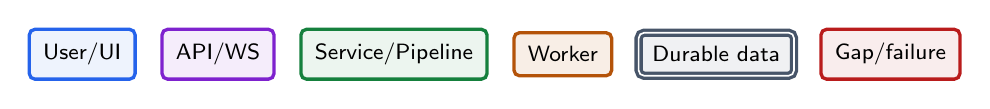
\begin{tikzpicture}[baseline=-.5ex]
\node[user,minimum height=5mm] (a) {User/UI};
\node[api,minimum height=5mm,right=3mm of a] (b) {API/WS};
\node[service,minimum height=5mm,right=3mm of b] (c) {Service/Pipeline};
\node[worker,minimum height=5mm,right=3mm of c] (d) {Worker};
\node[data,minimum height=5mm,right=3mm of d] (e) {Durable data};
\node[warning,minimum height=5mm,right=3mm of e] (f) {Gap/failure};
\end{tikzpicture}}

\begin{document}

% -----------------------------------------------------------------------------
\flowtitle{1. End-to-end system and responsibility flow}{Legend: \legend}
\resizebox{\textwidth}{0.82\textheight}{%
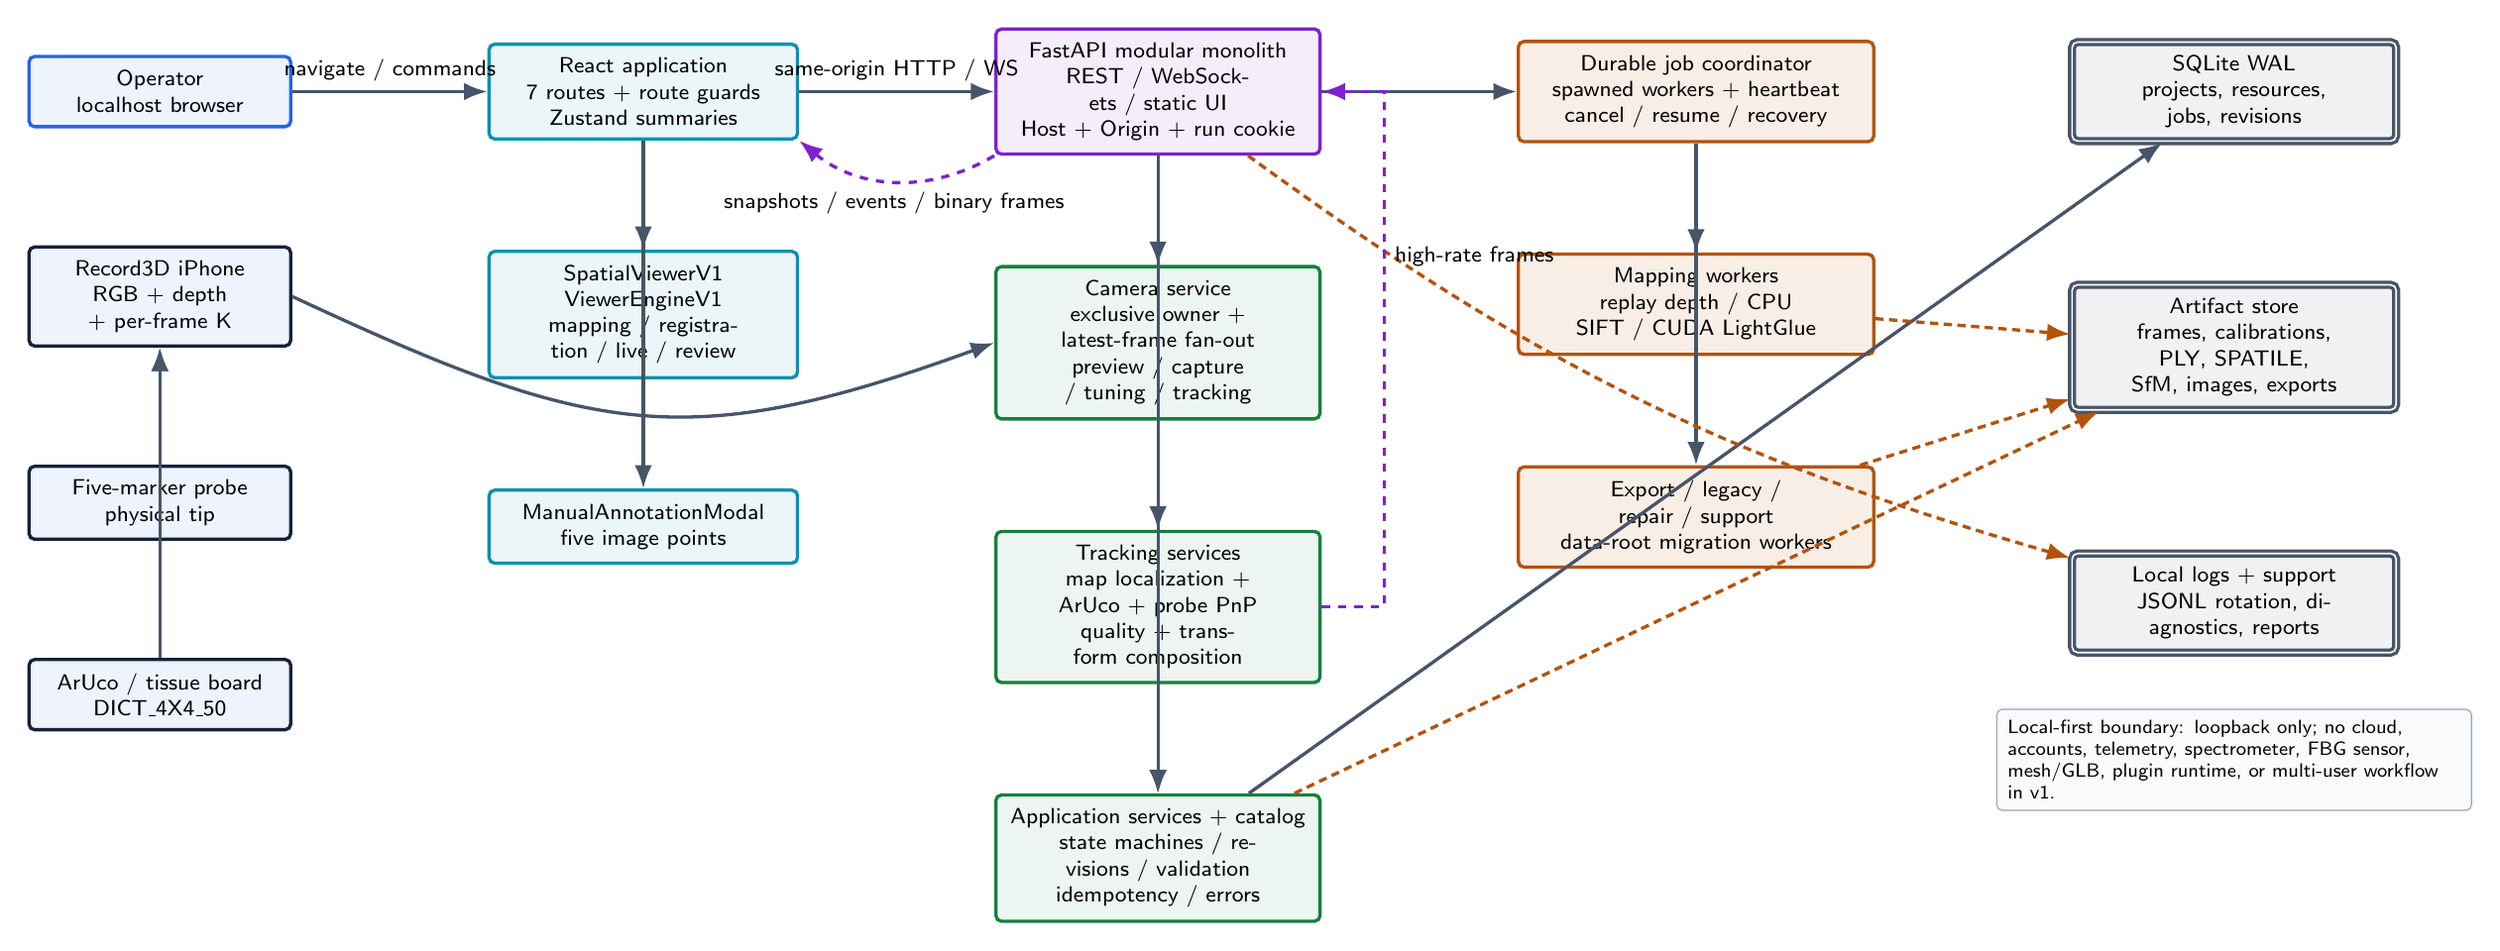
\begin{tikzpicture}[node distance=12mm and 18mm]
\node[user,text width=30mm] (operator) {Operator\\localhost browser};
\node[hardware,text width=30mm,below=15mm of operator] (iphone) {Record3D iPhone\\RGB + depth + per-frame K};
\node[hardware,text width=30mm,below=15mm of iphone] (probe) {Five-marker probe\\physical tip};
\node[hardware,text width=30mm,below=15mm of probe] (board) {ArUco / tissue board\\DICT\_4X4\_50};

\node[page,text width=36mm,right=25mm of operator] (react) {React application\\7 routes + route guards\\Zustand summaries};
\node[page,text width=36mm,below=14mm of react] (viewer) {SpatialViewerV1\\ViewerEngineV1\\mapping / registration / live / review};
\node[page,text width=36mm,below=14mm of viewer] (annotation) {ManualAnnotationModal\\five image points};

\node[api,text width=38mm,right=25mm of react] (fastapi) {FastAPI modular monolith\\REST / WebSockets / static UI\\Host + Origin + run cookie};
\node[service,text width=38mm,below=14mm of fastapi] (camera) {Camera service\\exclusive owner + latest-frame fan-out\\preview / capture / tuning / tracking};
\node[service,text width=38mm,below=14mm of camera] (tracking) {Tracking services\\map localization + ArUco + probe PnP\\quality + transform composition};
\node[service,text width=38mm,below=14mm of tracking] (catalog) {Application services + catalog\\state machines / revisions / validation\\idempotency / errors};

\node[worker,text width=42mm,right=25mm of fastapi] (jobs) {Durable job coordinator\\spawned workers + heartbeat\\cancel / resume / recovery};
\node[worker,text width=42mm,below=14mm of jobs] (compute) {Mapping workers\\replay depth / CPU SIFT / CUDA LightGlue};
\node[worker,text width=42mm,below=14mm of compute] (ops) {Export / legacy / repair / support\\data-root migration workers};

\node[data,text width=38mm,right=25mm of jobs] (sqlite) {SQLite WAL\\projects, resources, jobs, revisions};
\node[data,text width=38mm,below=18mm of sqlite] (artifacts) {Artifact store\\frames, calibrations, PLY, SPATILE,\\SfM, images, exports};
\node[data,text width=38mm,below=18mm of artifacts] (logs) {Local logs + support\\JSONL rotation, diagnostics, reports};

\draw[flow] (operator) -- node[above]{navigate / commands} (react);
\draw[flow] (react) -- node[above]{same-origin HTTP / WS} (fastapi);
\draw[event] (fastapi.south west) to[bend left=35] node[below]{snapshots / events / binary frames} (react.south east);
\draw[flow] (react) -- (viewer);
\draw[flow] (react) -- (annotation);
\draw[flow] (iphone.east) to[out=-25,in=200,looseness=1.2] (camera.west);
\draw[flow] (probe) -- (iphone);
\draw[flow] (board) -- (iphone);
\draw[flow] (fastapi) -- (camera);
\draw[flow] (camera) -- (tracking);
\draw[flow] (tracking) -- (catalog);
\draw[flow] (fastapi) -- (catalog);
\draw[flow] (fastapi) -- (jobs);
\draw[flow] (jobs) -- (compute);
\draw[flow] (jobs) -- (ops);
\draw[flow] (catalog) -- (sqlite);
\draw[artifact] (compute) -- (artifacts);
\draw[artifact] (ops) -- (artifacts);
\draw[artifact] (catalog) -- (artifacts);
\draw[artifact] (fastapi) to[bend right=10] (logs);
\draw[event] (tracking.east) -- ++(8mm,0) |- node[pos=.34,right]{high-rate frames} (fastapi.east);

\node[note,text width=58mm,below=7mm of logs] {Local-first boundary: loopback only; no cloud, accounts, telemetry, spectrometer, FBG sensor, mesh/GLB, plugin runtime, or multi-user workflow in v1.};
\end{tikzpicture}}
\newpage

% -----------------------------------------------------------------------------
\flowtitle{2. User navigation, route guards, and project lifecycle}{Primary task order and every application page}
\resizebox{\textwidth}{0.82\textheight}{%
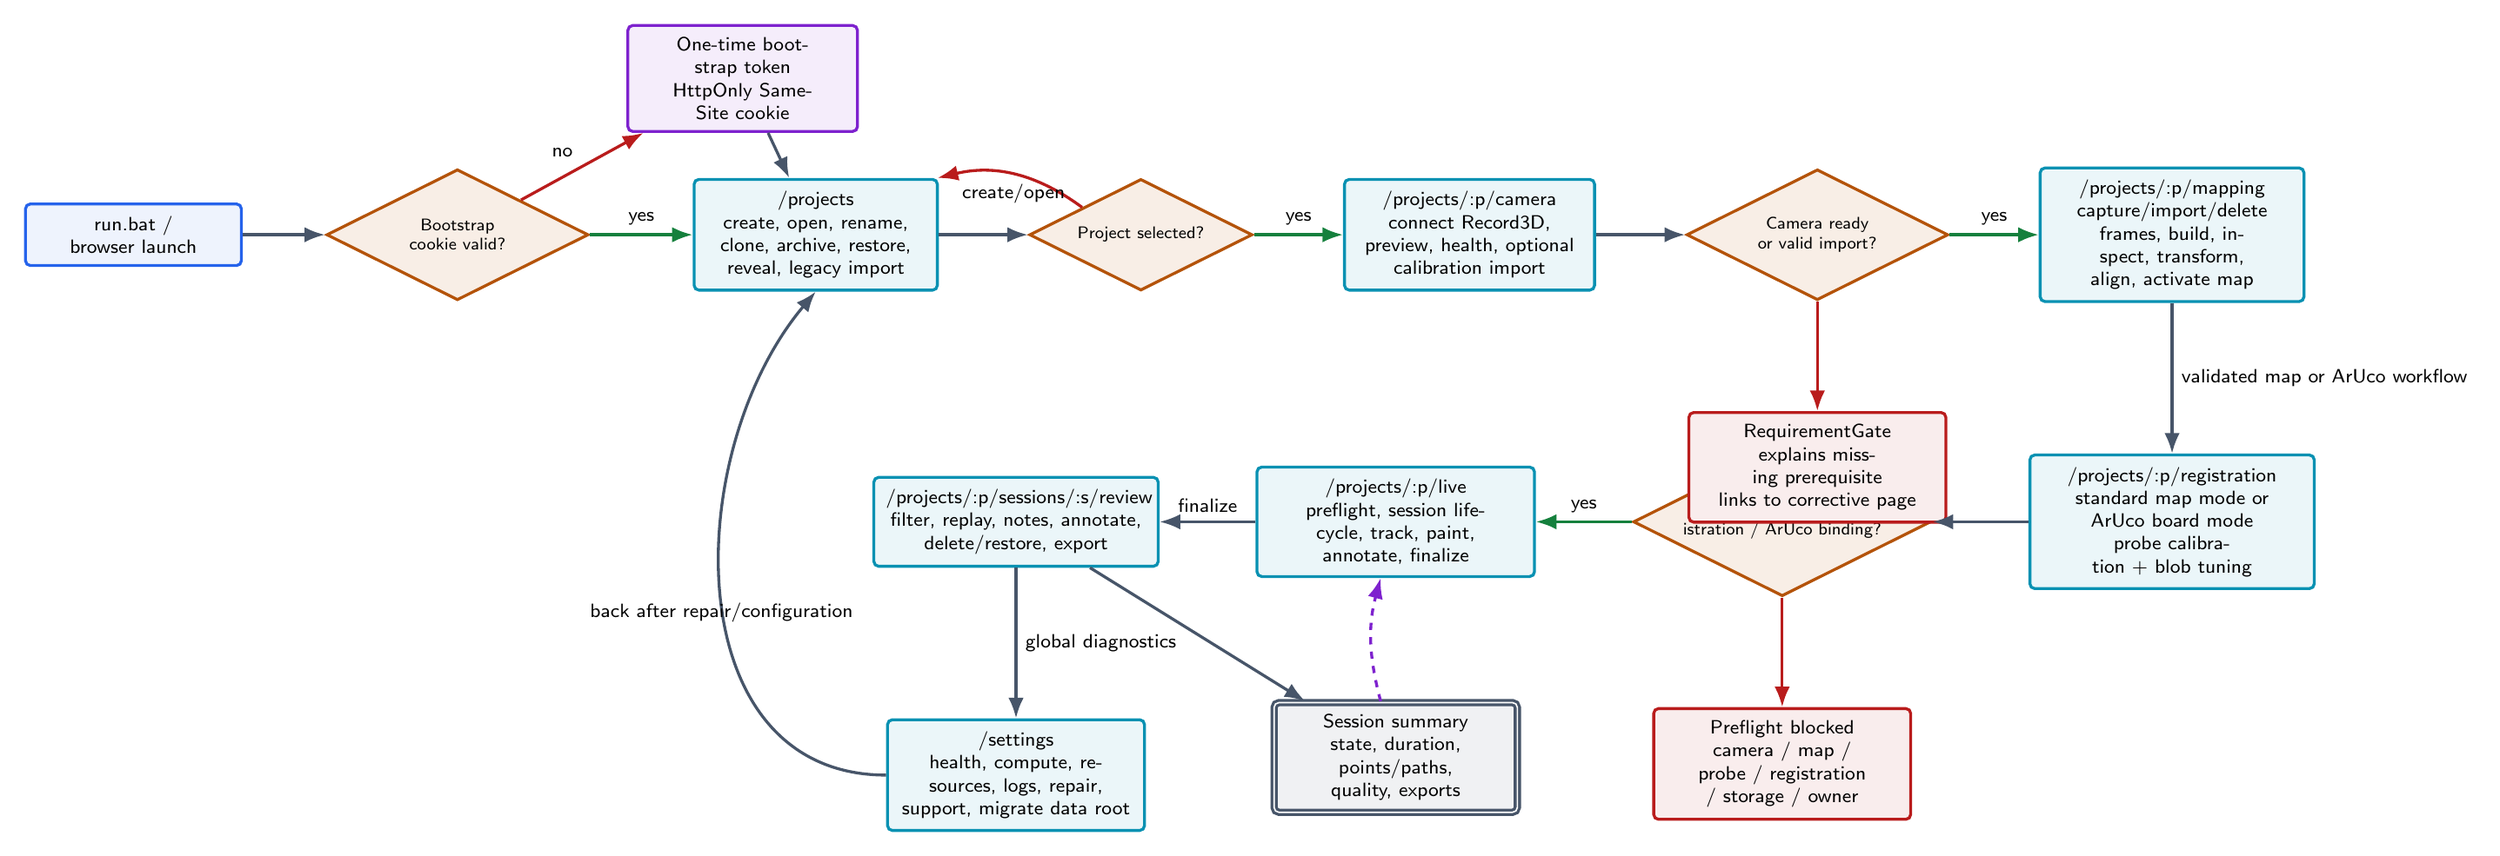
\begin{tikzpicture}[node distance=11mm and 13mm]
\node[user,text width=28mm] (launch) {run.bat / browser launch};
\node[decision,text width=25mm,right=12mm of launch] (boot) {Bootstrap cookie valid?};
\node[api,text width=30mm,above right=10mm and 15mm of boot] (bootstrap) {One-time bootstrap token\\HttpOnly SameSite cookie};
\node[page,text width=32mm,right=15mm of boot] (projects) {/projects\\create, open, rename, clone, archive, restore, reveal, legacy import};
\node[decision,text width=24mm,right=13mm of projects] (selected) {Project selected?};
\node[page,text width=33mm,right=13mm of selected] (camera) {/projects/:p/camera\\connect Record3D, preview, health, optional calibration import};
\node[decision,text width=24mm,right=13mm of camera] (camready) {Camera ready or valid import?};
\node[page,text width=35mm,right=13mm of camready] (mapping) {/projects/:p/mapping\\capture/import/delete frames, build, inspect, transform, align, activate map};

\node[page,text width=38mm,below=22mm of mapping] (registration) {/projects/:p/registration\\standard map mode or ArUco board mode\\probe calibration + blob tuning};
\node[decision,text width=29mm,left=14mm of registration] (regready) {Active probe + valid registration / ArUco binding?};
\node[page,text width=37mm,left=14mm of regready] (live) {/projects/:p/live\\preflight, session lifecycle, track, paint, annotate, finalize};
\node[page,text width=38mm,left=14mm of live] (review) {/projects/:p/sessions/:s/review\\filter, replay, notes, annotate, delete/restore, export};
\node[page,text width=34mm,below=22mm of review] (settings) {/settings\\health, compute, resources, logs, repair, support, migrate data root};

\node[warning,text width=34mm,below=16mm of camready] (guard1) {RequirementGate\\explains missing prerequisite\\links to corrective page};
\node[warning,text width=34mm,below=16mm of regready] (guard2) {Preflight blocked\\camera / map / probe / registration / storage / owner};
\node[data,text width=32mm,below=18mm of live] (sessiondata) {Session summary\\state, duration, points/paths, quality, exports};

\draw[flow] (launch) -- (boot);
\draw[no] (boot) -- node[above left]{no} (bootstrap);
\draw[flow] (bootstrap) -- (projects);
\draw[yes] (boot) -- node[above]{yes} (projects);
\draw[flow] (projects) -- (selected);
\draw[yes] (selected) -- node[above]{yes} (camera);
\draw[no] (selected) to[bend right=25] node[below]{create/open} (projects);
\draw[flow] (camera) -- (camready);
\draw[yes] (camready) -- node[above]{yes} (mapping);
\draw[no] (camready) -- (guard1);
\draw[flow] (mapping) -- node[right]{validated map or ArUco workflow} (registration);
\draw[flow] (registration) -- (regready);
\draw[yes] (regready) -- node[above]{yes} (live);
\draw[no] (regready) -- (guard2);
\draw[flow] (live) -- node[above]{finalize} (review);
\draw[flow] (review) -- node[right]{global diagnostics} (settings);
\draw[flow] (review) -- (sessiondata);
\draw[event] (sessiondata) to[bend left=15] (live);
\draw[flow] (settings.west) to[out=180,in=230,looseness=1.1] node[below]{back after repair/configuration} (projects.south);
\end{tikzpicture}}
\newpage

% -----------------------------------------------------------------------------
\flowtitle{3. Camera setup, normalized frames, capture sets, and frame management}{Record3D is primary; external calibration is import-only}
\resizebox{\textwidth}{0.82\textheight}{%
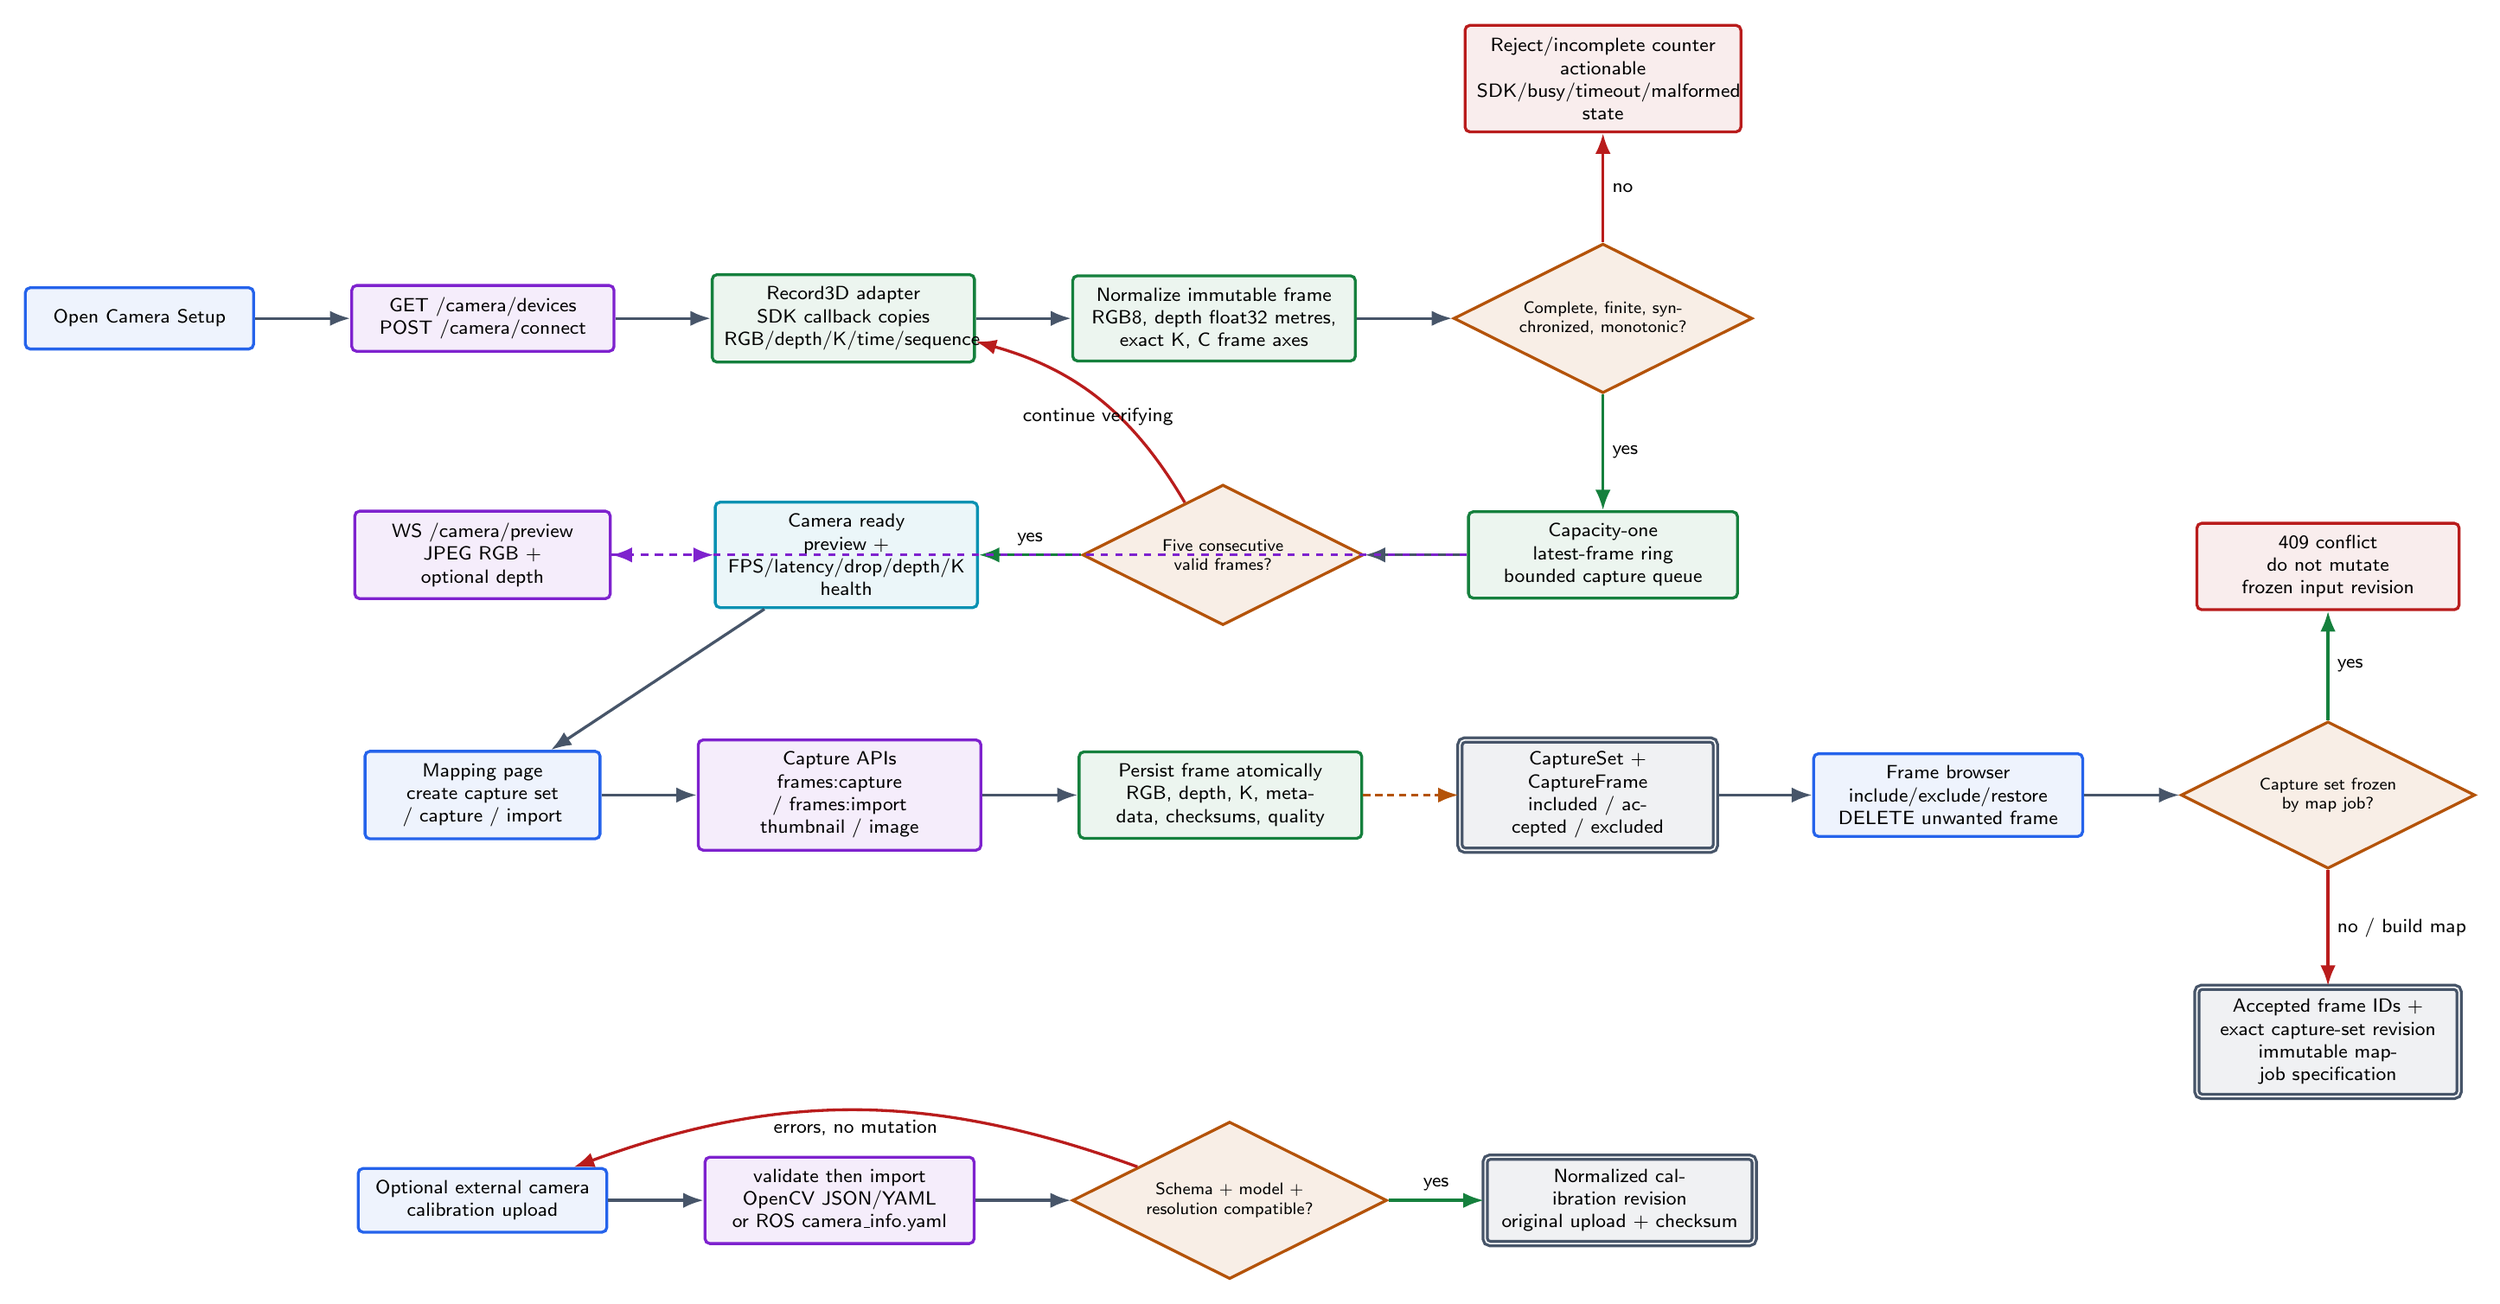
\begin{tikzpicture}[node distance=10mm and 13mm]
\node[user,text width=30mm] (open) {Open Camera Setup};
\node[api,text width=35mm,right=14mm of open] (enumerate) {GET /camera/devices\\POST /camera/connect};
\node[service,text width=35mm,right=14mm of enumerate] (adapter) {Record3D adapter\\SDK callback copies RGB/depth/K/time/sequence};
\node[service,text width=38mm,right=14mm of adapter] (normalize) {Normalize immutable frame\\RGB8, depth float32 metres, exact K, C frame axes};
\node[decision,text width=30mm,right=14mm of normalize] (valid) {Complete, finite, synchronized, monotonic?};

\node[warning,text width=37mm,above=16mm of valid] (reject) {Reject/incomplete counter\\actionable SDK/busy/timeout/malformed state};
\node[service,text width=36mm,below=17mm of valid] (ring) {Capacity-one latest-frame ring\\bounded capture queue};
\node[decision,text width=28mm,left=15mm of ring] (five) {Five consecutive valid frames?};
\node[page,text width=35mm,left=15mm of five] (ready) {Camera ready\\preview + FPS/latency/drop/depth/K health};
\node[api,text width=34mm,left=15mm of ready] (preview) {WS /camera/preview\\JPEG RGB + optional depth};

\node[user,text width=31mm,below=22mm of preview] (capturecmd) {Mapping page\\create capture set / capture / import};
\node[api,text width=38mm,right=14mm of capturecmd] (captureapi) {Capture APIs\\frames:capture / frames:import\\thumbnail / image};
\node[service,text width=38mm,right=14mm of captureapi] (persist) {Persist frame atomically\\RGB, depth, K, metadata, checksums, quality};
\node[data,text width=34mm,right=14mm of persist] (frames) {CaptureSet + CaptureFrame\\included / accepted / excluded};
\node[user,text width=36mm,right=14mm of frames] (manage) {Frame browser\\include/exclude/restore\\DELETE unwanted frame};
\node[decision,text width=29mm,right=14mm of manage] (frozen) {Capture set frozen by map job?};
\node[warning,text width=35mm,above=16mm of frozen] (conflict) {409 conflict\\do not mutate frozen input revision};
\node[data,text width=35mm,below=17mm of frozen] (revision) {Accepted frame IDs + exact capture-set revision\\immutable map-job specification};

\node[user,text width=33mm,below=48mm of capturecmd] (external) {Optional external camera calibration upload};
\node[api,text width=36mm,right=14mm of external] (calval) {validate then import\\OpenCV JSON/YAML or ROS camera\_info.yaml};
\node[decision,text width=32mm,right=14mm of calval] (compat) {Schema + model + resolution compatible?};
\node[data,text width=36mm,right=14mm of compat] (caldata) {Normalized calibration revision\\original upload + checksum};

\draw[flow] (open) -- (enumerate);
\draw[flow] (enumerate) -- (adapter);
\draw[flow] (adapter) -- (normalize);
\draw[flow] (normalize) -- (valid);
\draw[no] (valid) -- node[right]{no} (reject);
\draw[yes] (valid) -- node[right]{yes} (ring);
\draw[flow] (ring) -- (five);
\draw[yes] (five) -- node[above]{yes} (ready);
\draw[no] (five) to[bend right=22] node[below]{continue verifying} (adapter);
\draw[event] (ring) -- (preview);
\draw[event] (preview) -- (ready);
\draw[flow] (ready) -- (capturecmd);
\draw[flow] (capturecmd) -- (captureapi);
\draw[flow] (captureapi) -- (persist);
\draw[artifact] (persist) -- (frames);
\draw[flow] (frames) -- (manage);
\draw[flow] (manage) -- (frozen);
\draw[yes] (frozen) -- node[right]{yes} (conflict);
\draw[no] (frozen) -- node[right]{no / build map} (revision);
\draw[flow] (external) -- (calval);
\draw[flow] (calval) -- (compat);
\draw[yes] (compat) -- node[above]{yes} (caldata);
\draw[no] (compat) to[bend right=20] node[below]{errors, no mutation} (external);
\end{tikzpicture}}
\newpage

% -----------------------------------------------------------------------------
\flowtitle{4. Mapping dispatch, reconstruction profiles, publication, and browser LOD}{No silent algorithm substitution inside an attempt}
\resizebox{\textwidth}{0.82\textheight}{%
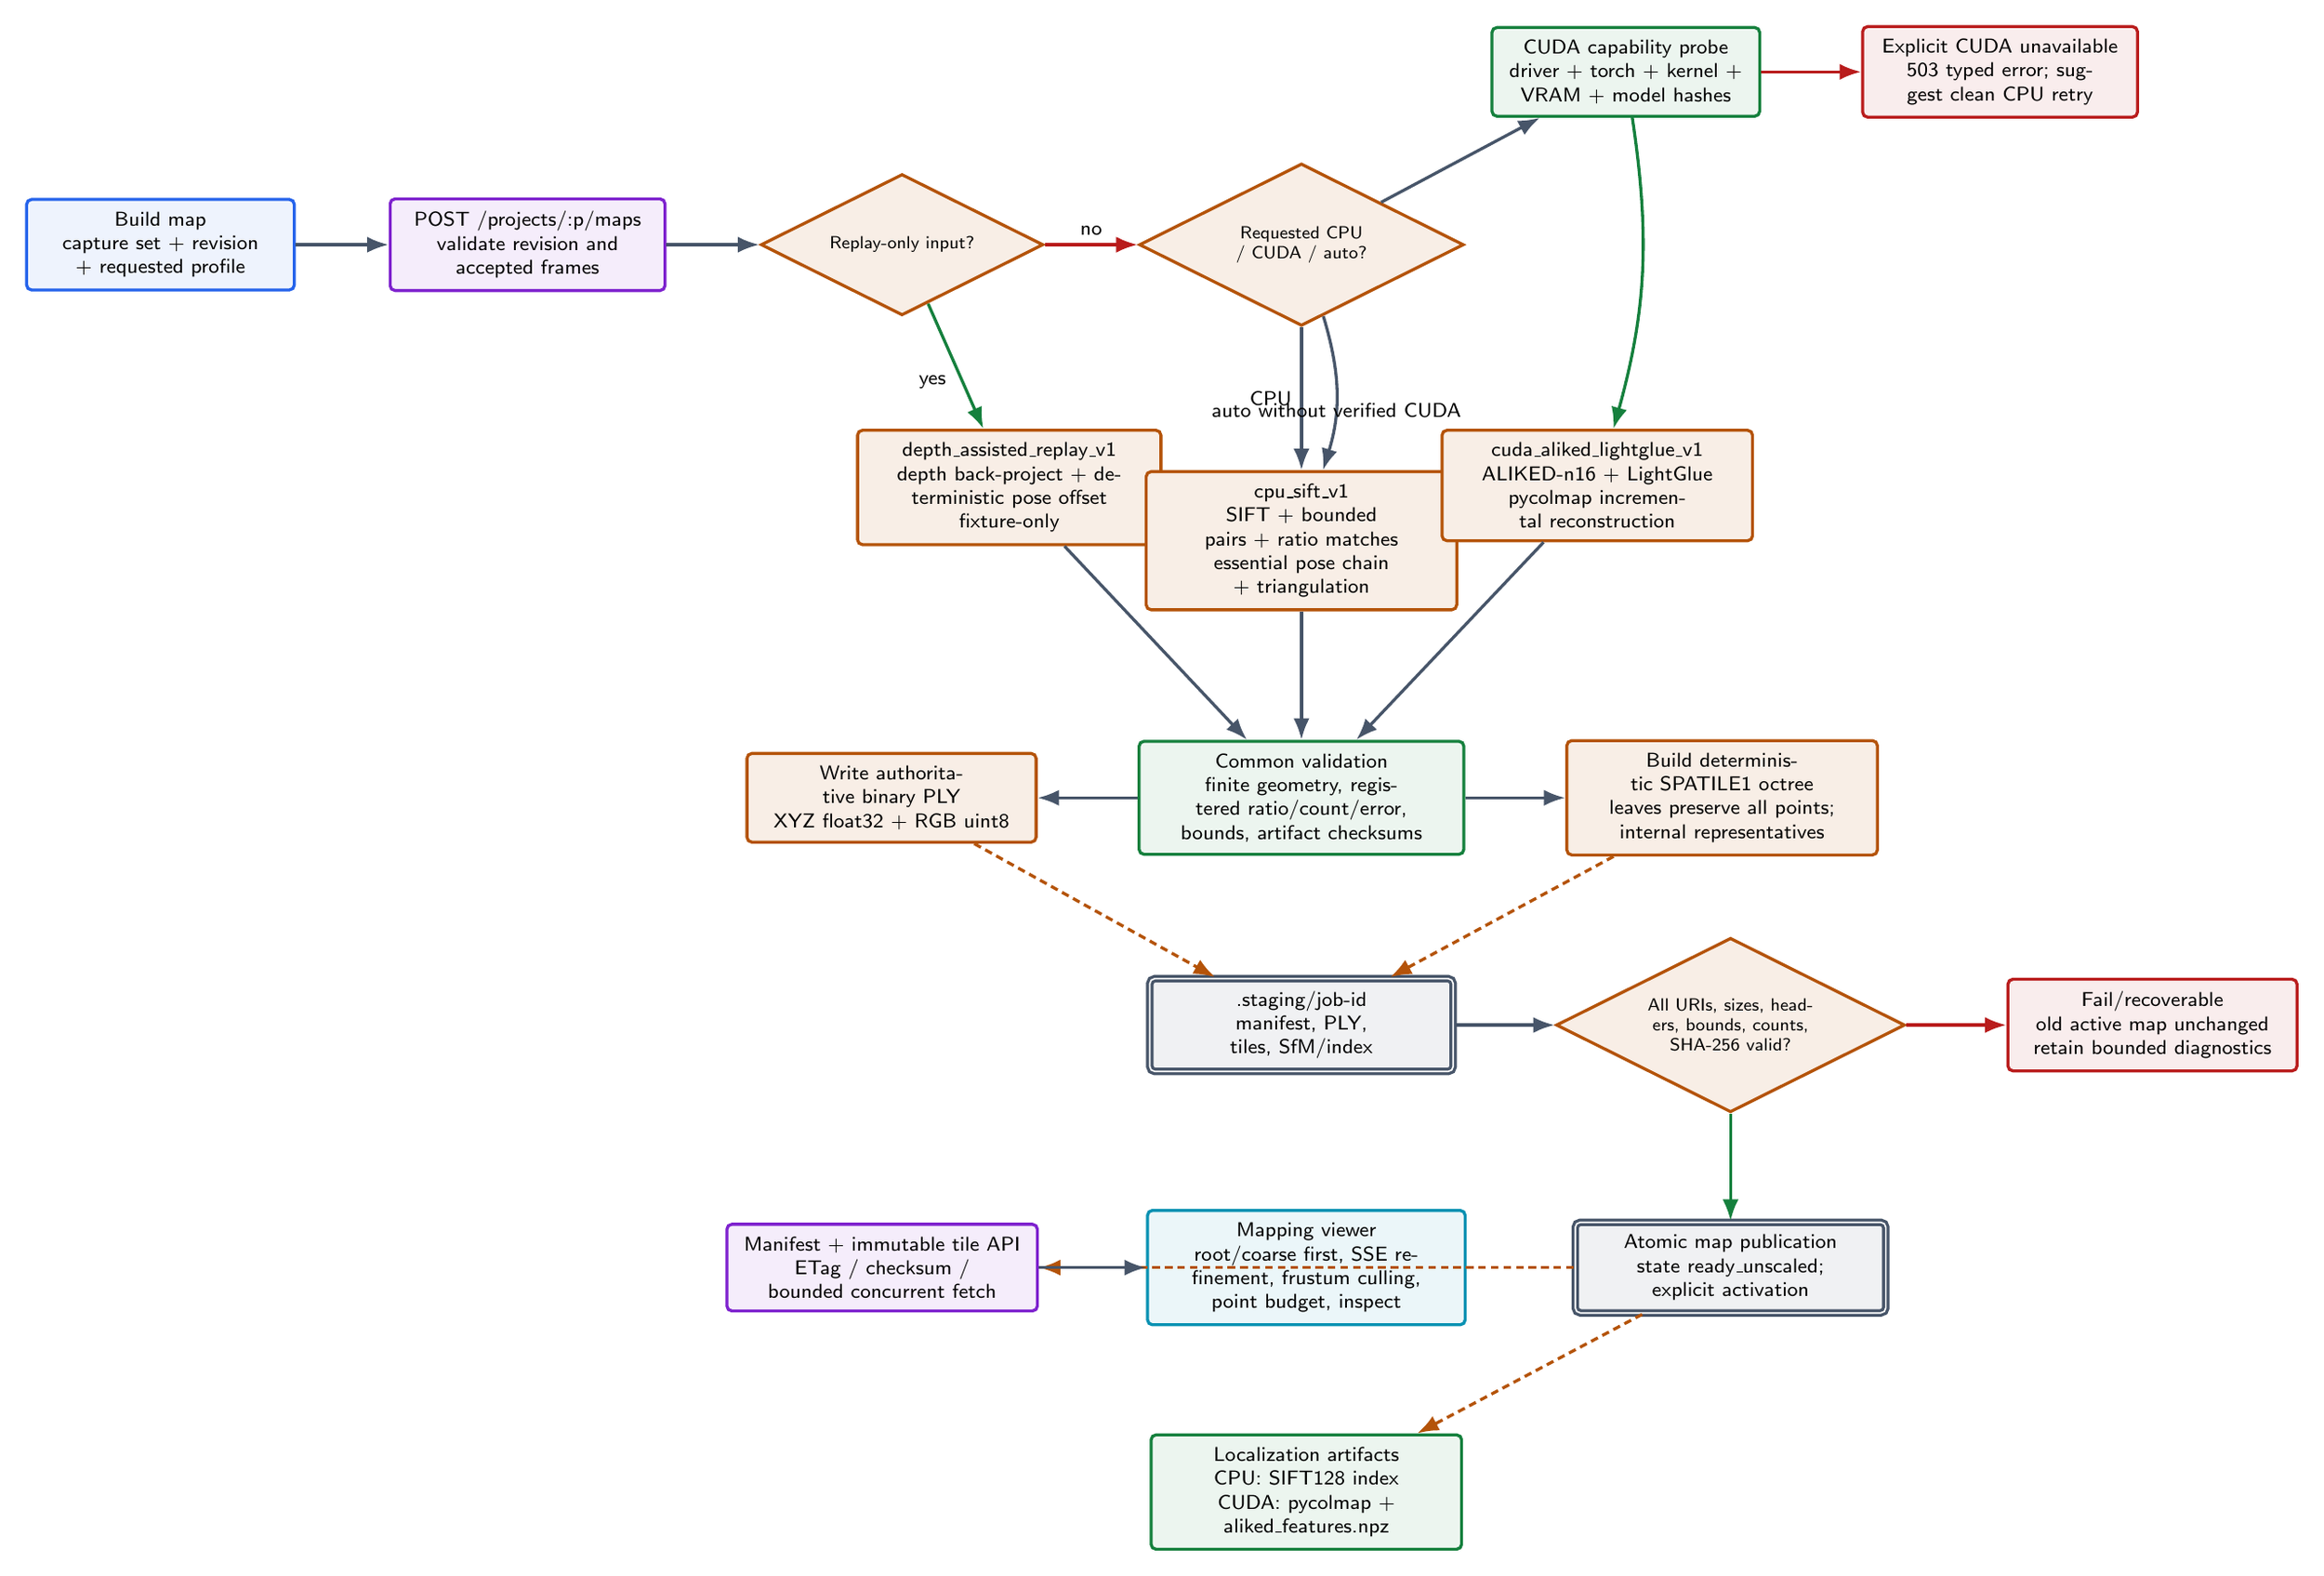
\begin{tikzpicture}[node distance=9mm and 12mm]
\node[user,text width=34mm] (build) {Build map\\capture set + revision + requested profile};
\node[api,text width=35mm,right=13mm of build] (mapapi) {POST /projects/:p/maps\\validate revision and accepted frames};
\node[decision,text width=31mm,right=13mm of mapapi] (source) {Replay-only input?};
\node[decision,text width=31mm,right=13mm of source] (profile) {Requested CPU / CUDA / auto?};
\node[service,text width=34mm,above right=12mm and 15mm of profile] (cudaProbe) {CUDA capability probe\\driver + torch + kernel + VRAM + model hashes};
\node[warning,text width=35mm,right=14mm of cudaProbe] (cudaerr) {Explicit CUDA unavailable\\503 typed error; suggest clean CPU retry};

\node[worker,text width=39mm,below left=20mm and 8mm of profile] (replay) {depth\_assisted\_replay\_v1\\depth back-project + deterministic pose offset\\fixture-only};
\node[worker,text width=40mm,below=20mm of profile] (cpu) {cpu\_sift\_v1\\SIFT + bounded pairs + ratio matches\\essential pose chain + triangulation};
\node[worker,text width=40mm,below right=20mm and 8mm of profile] (cuda) {cuda\_aliked\_lightglue\_v1\\ALIKED-n16 + LightGlue\\pycolmap incremental reconstruction};

\node[service,text width=42mm,below=18mm of cpu] (validate) {Common validation\\finite geometry, registered ratio/count/error, bounds, artifact checksums};
\node[worker,text width=37mm,left=14mm of validate] (ply) {Write authoritative binary PLY\\XYZ float32 + RGB uint8};
\node[worker,text width=40mm,right=14mm of validate] (tiles) {Build deterministic SPATILE1 octree\\leaves preserve all points; internal representatives};
\node[data,text width=39mm,below=17mm of validate] (staging) {.staging/job-id\\manifest, PLY, tiles, SfM/index};
\node[decision,text width=30mm,right=14mm of staging] (publishok) {All URIs, sizes, headers, bounds, counts, SHA-256 valid?};
\node[warning,text width=37mm,right=14mm of publishok] (fail) {Fail/recoverable\\old active map unchanged\\retain bounded diagnostics};
\node[data,text width=40mm,below=15mm of publishok] (published) {Atomic map publication\\state ready\_unscaled; explicit activation};
\node[page,text width=41mm,left=15mm of published] (viewer) {Mapping viewer\\root/coarse first, SSE refinement, frustum culling, point budget, inspect};
\node[api,text width=40mm,left=15mm of viewer] (tileapi) {Manifest + immutable tile API\\ETag / checksum / bounded concurrent fetch};
\node[service,text width=40mm,below=15mm of viewer] (localidx) {Localization artifacts\\CPU: SIFT128 index\\CUDA: pycolmap + aliked\_features.npz};

\draw[flow] (build) -- (mapapi);
\draw[flow] (mapapi) -- (source);
\draw[yes] (source) -- node[below left]{yes} (replay);
\draw[no] (source) -- node[above]{no} (profile);
\draw[flow] (profile) -- (cudaProbe);
\draw[no] (cudaProbe) -- (cudaerr);
\draw[yes] (cudaProbe) to[bend left=12] (cuda);
\draw[flow] (profile) -- node[left]{CPU} (cpu);
\draw[flow] (profile) to[bend left=17] node[below]{auto without verified CUDA} (cpu);
\draw[flow] (replay) -- (validate);
\draw[flow] (cpu) -- (validate);
\draw[flow] (cuda) -- (validate);
\draw[flow] (validate) -- (ply);
\draw[flow] (validate) -- (tiles);
\draw[artifact] (ply) -- (staging);
\draw[artifact] (tiles) -- (staging);
\draw[flow] (staging) -- (publishok);
\draw[no] (publishok) -- (fail);
\draw[yes] (publishok) -- (published);
\draw[artifact] (published) -- (tileapi);
\draw[flow] (tileapi) -- (viewer);
\draw[artifact] (published) -- (localidx);
\end{tikzpicture}}
\newpage

% -----------------------------------------------------------------------------
\flowtitle{5. Probe calibration, reusable JSON, tracking test, and blob-detector tuning}{The ``Can't track the probe?'' subsection is modal and draft-safe}
\resizebox{\textwidth}{0.82\textheight}{%
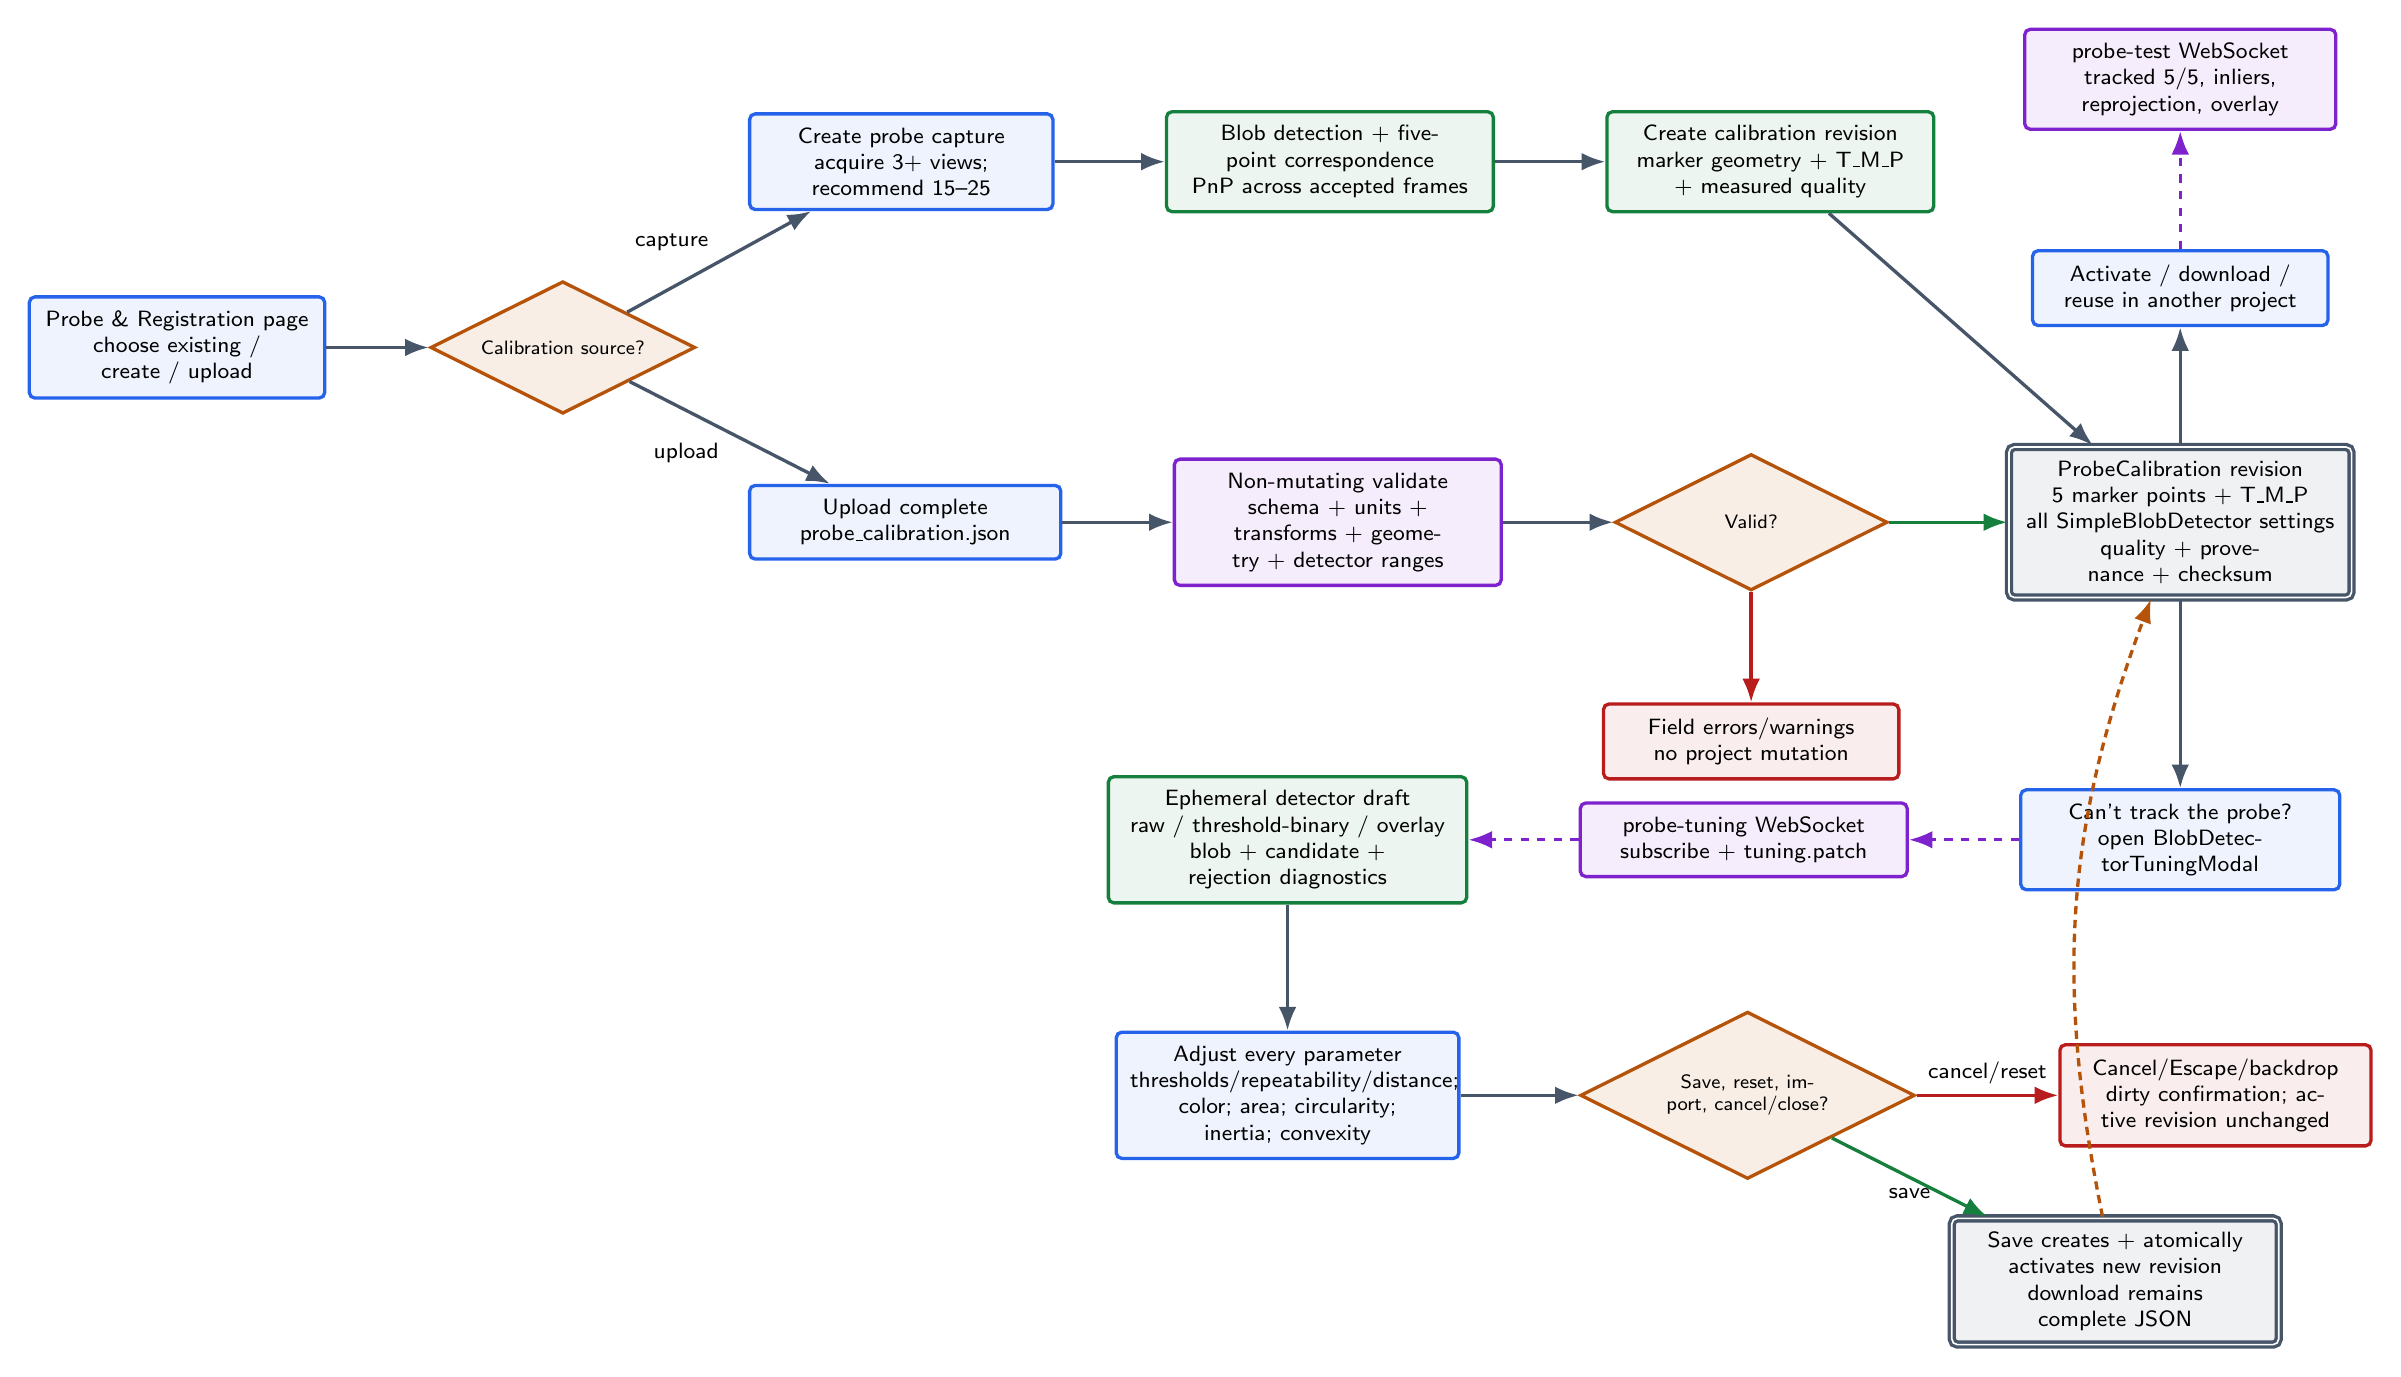
\begin{tikzpicture}[node distance=10mm and 13mm]
\node[user,text width=34mm] (entry) {Probe \& Registration page\\choose existing / create / upload};
\node[decision,text width=26mm,right=13mm of entry] (choice) {Calibration source?};

\node[user,text width=35mm,above right=13mm and 15mm of choice] (capture) {Create probe capture\\acquire 3+ views; recommend 15--25};
\node[service,text width=38mm,right=14mm of capture] (detect) {Blob detection + five-point correspondence\\PnP across accepted frames};
\node[service,text width=38mm,right=14mm of detect] (opt) {Create calibration revision\\marker geometry + T\_M\_P + measured quality};

\node[user,text width=36mm,below right=13mm and 15mm of choice] (upload) {Upload complete probe\_calibration.json};
\node[api,text width=38mm,right=14mm of upload] (validate) {Non-mutating validate\\schema + units + transforms + geometry + detector ranges};
\node[decision,text width=27mm,right=14mm of validate] (valid) {Valid?};
\node[warning,text width=34mm,below=14mm of valid] (errors) {Field errors/warnings\\no project mutation};

\node[data,text width=40mm,right=15mm of valid] (cal) {ProbeCalibration revision\\5 marker points + T\_M\_P\\all SimpleBlobDetector settings\\quality + provenance + checksum};
\node[user,text width=34mm,above=15mm of cal] (activate) {Activate / download / reuse in another project};
\node[api,text width=36mm,above=15mm of activate] (testws) {probe-test WebSocket\\tracked 5/5, inliers, reprojection, overlay};

\node[user,text width=37mm,below=24mm of cal] (cant) {Can't track the probe?\\open BlobDetectorTuningModal};
\node[api,text width=38mm,left=14mm of cant] (tuningws) {probe-tuning WebSocket\\subscribe + tuning.patch};
\node[service,text width=42mm,left=14mm of tuningws] (draft) {Ephemeral detector draft\\raw / threshold-binary / overlay\\blob + candidate + rejection diagnostics};
\node[user,text width=40mm,below=16mm of draft] (params) {Adjust every parameter\\thresholds/repeatability/distance; color; area; circularity; inertia; convexity};
\node[decision,text width=28mm,right=15mm of params] (close) {Save, reset, import, cancel/close?};
\node[warning,text width=36mm,right=18mm of close] (discard) {Cancel/Escape/backdrop\\dirty confirmation; active revision unchanged};
\node[data,text width=38mm,below right=10mm and 15mm of close] (revision) {Save creates + atomically activates new revision\\download remains complete JSON};

\draw[flow] (entry) -- (choice);
\draw[flow] (choice) -- node[above left]{capture} (capture);
\draw[flow] (capture) -- (detect);
\draw[flow] (detect) -- (opt);
\draw[flow] (opt) -- (cal);
\draw[flow] (choice) -- node[below left]{upload} (upload);
\draw[flow] (upload) -- (validate);
\draw[flow] (validate) -- (valid);
\draw[no] (valid) -- (errors);
\draw[yes] (valid) -- (cal);
\draw[flow] (cal) -- (activate);
\draw[event] (activate) -- (testws);
\draw[flow] (cal) -- (cant);
\draw[event] (cant) -- (tuningws);
\draw[event] (tuningws) -- (draft);
\draw[flow] (draft) -- (params);
\draw[flow] (params) -- (close);
\draw[no] (close) -- node[above]{cancel/reset} (discard);
\draw[yes] (close) -- node[below]{save} (revision);
\draw[artifact] (revision) to[bend left=16] (cal);
\end{tikzpicture}}
\newpage

% -----------------------------------------------------------------------------
\flowtitle{6. Registration logic: standard map mode and ArUco board mode}{Both routes bind probe geometry to a physical reference frame}
\resizebox{\textwidth}{0.82\textheight}{%
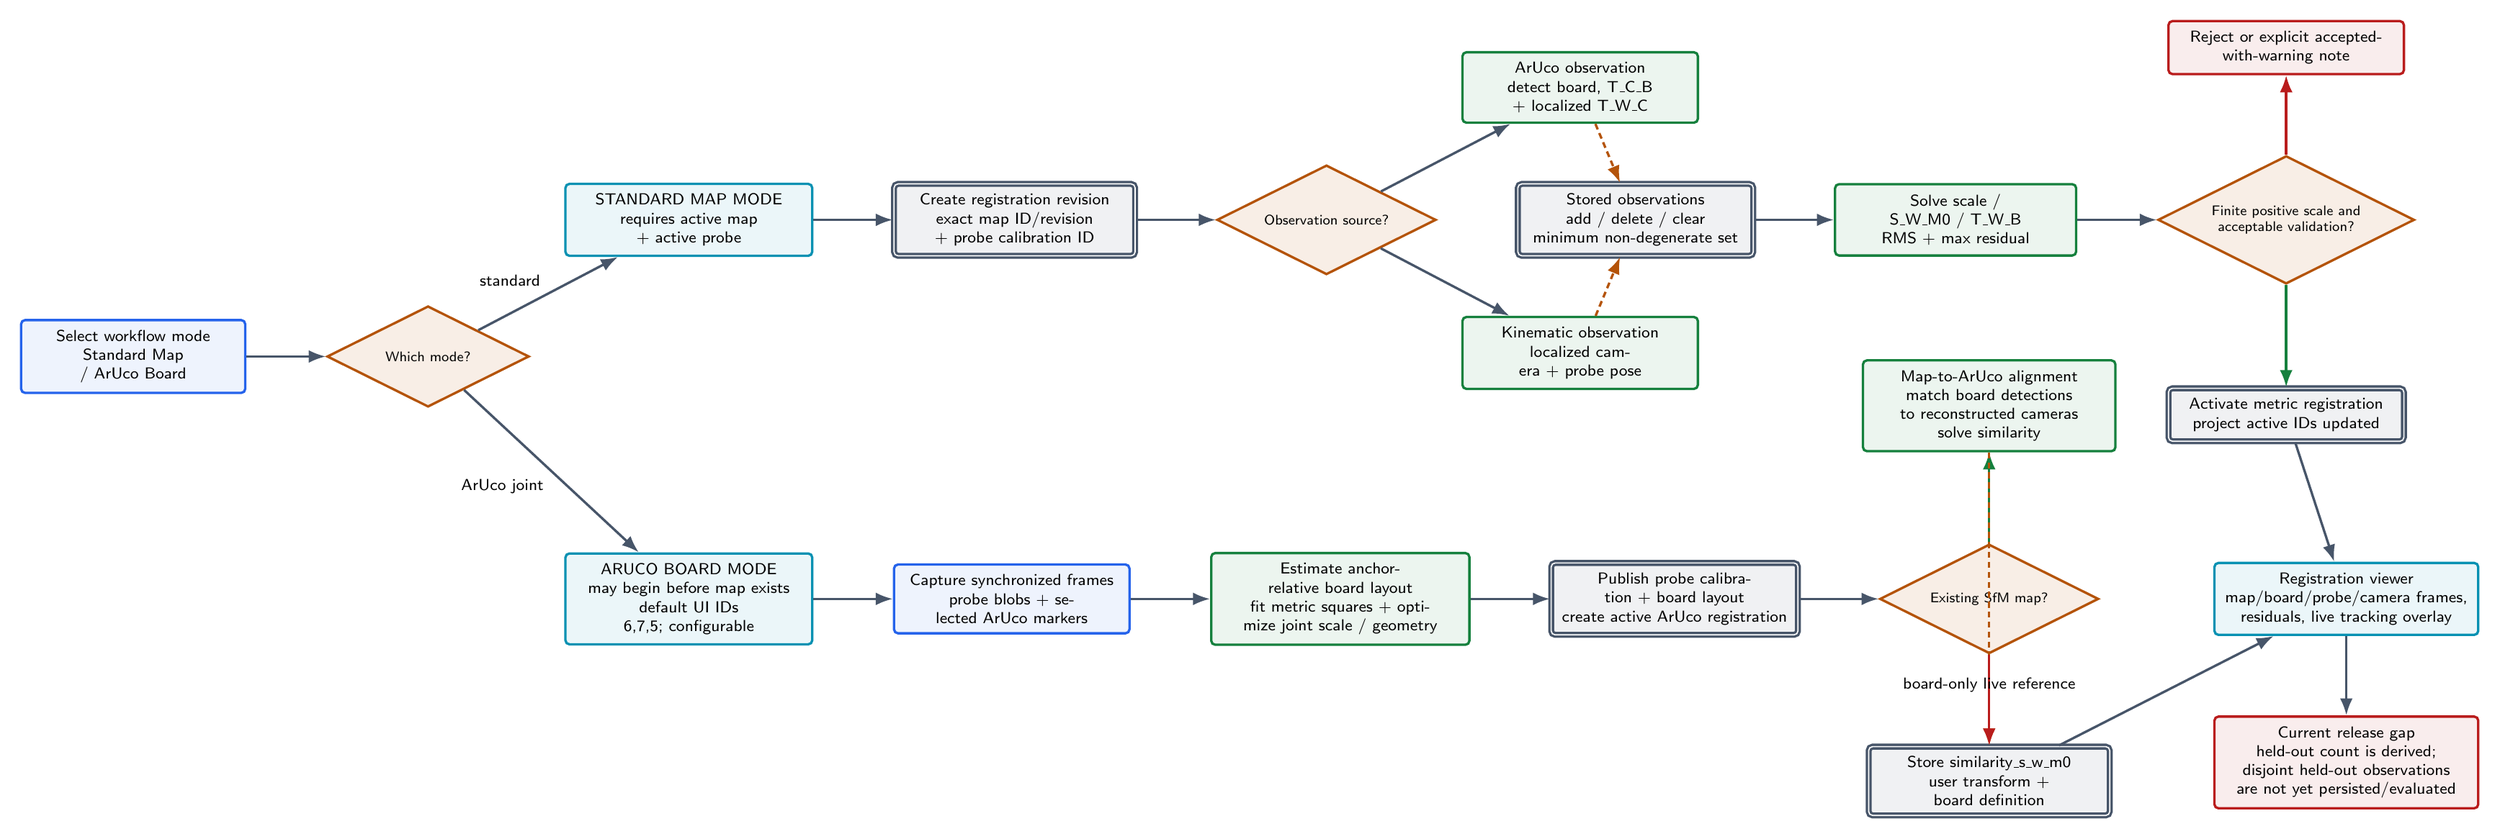
\begin{tikzpicture}[node distance=9mm and 13mm]
\node[user,text width=36mm] (mode) {Select workflow mode\\Standard Map / ArUco Board};
\node[decision,text width=28mm,right=14mm of mode] (which) {Which mode?};

\node[page,text width=40mm,above right=13mm and 15mm of which] (standard) {STANDARD MAP MODE\\requires active map + active probe};
\node[data,text width=39mm,right=14mm of standard] (regrev) {Create registration revision\\exact map ID/revision + probe calibration ID};
\node[decision,text width=31mm,right=14mm of regrev] (obsmode) {Observation source?};
\node[service,text width=38mm,above right=12mm and 14mm of obsmode] (arucoobs) {ArUco observation\\detect board, T\_C\_B + localized T\_W\_C};
\node[service,text width=38mm,below right=12mm and 14mm of obsmode] (kinobs) {Kinematic observation\\localized camera + probe pose};
\node[data,text width=38mm,right=14mm of obsmode] (observations) {Stored observations\\add / delete / clear\\minimum non-degenerate set};
\node[service,text width=39mm,right=14mm of observations] (solve) {Solve scale / S\_W\_M0 / T\_W\_B\\RMS + max residual};
\node[decision,text width=31mm,right=14mm of solve] (valreg) {Finite positive scale and acceptable validation?};
\node[warning,text width=38mm,above=14mm of valreg] (regwarn) {Reject or explicit accepted-with-warning note};
\node[data,text width=38mm,below=18mm of valreg] (active) {Activate metric registration\\project active IDs updated};

\node[page,text width=40mm,below right=30mm and 15mm of which] (joint) {ARUCO BOARD MODE\\may begin before map exists\\default UI IDs 6,7,5; configurable};
\node[user,text width=38mm,right=14mm of joint] (jointcap) {Capture synchronized frames\\probe blobs + selected ArUco markers};
\node[service,text width=42mm,right=14mm of jointcap] (jointsolve) {Estimate anchor-relative board layout\\fit metric squares + optimize joint scale / geometry};
\node[data,text width=40mm,right=14mm of jointsolve] (jointcal) {Publish probe calibration + board layout\\create active ArUco registration};
\node[decision,text width=30mm,right=14mm of jointcal] (hasmap) {Existing SfM map?};
\node[service,text width=41mm,above=16mm of hasmap] (align) {Map-to-ArUco alignment\\match board detections to reconstructed cameras\\solve similarity};
\node[data,text width=39mm,below=16mm of hasmap] (similarity) {Store similarity\_s\_w\_m0\\user transform + board definition};

\node[page,text width=43mm,right=20mm of hasmap] (regviewer) {Registration viewer\\map/board/probe/camera frames, residuals, live tracking overlay};
\node[warning,text width=43mm,below=14mm of regviewer] (gap) {Current release gap\\held-out count is derived; disjoint held-out observations are not yet persisted/evaluated};

\draw[flow] (mode) -- (which);
\draw[flow] (which) -- node[above left]{standard} (standard);
\draw[flow] (standard) -- (regrev);
\draw[flow] (regrev) -- (obsmode);
\draw[flow] (obsmode) -- (arucoobs);
\draw[flow] (obsmode) -- (kinobs);
\draw[artifact] (arucoobs) -- (observations);
\draw[artifact] (kinobs) -- (observations);
\draw[flow] (observations) -- (solve);
\draw[flow] (solve) -- (valreg);
\draw[no] (valreg) -- (regwarn);
\draw[yes] (valreg) -- (active);
\draw[flow] (which) -- node[below left]{ArUco joint} (joint);
\draw[flow] (joint) -- (jointcap);
\draw[flow] (jointcap) -- (jointsolve);
\draw[flow] (jointsolve) -- (jointcal);
\draw[flow] (jointcal) -- (hasmap);
\draw[yes] (hasmap) -- (align);
\draw[artifact] (align) -- (similarity);
\draw[no] (hasmap) -- node[above]{board-only live reference} (similarity);
\draw[flow] (active) -- (regviewer);
\draw[flow] (similarity) -- (regviewer);
\draw[flow] (regviewer) -- (gap);
\end{tikzpicture}}
\newpage

% -----------------------------------------------------------------------------
\flowtitle{7. Live session preflight, localization, probe-tip composition, and painting}{High-rate frames are ephemeral; paint records are durable}
\resizebox{\textwidth}{0.82\textheight}{%
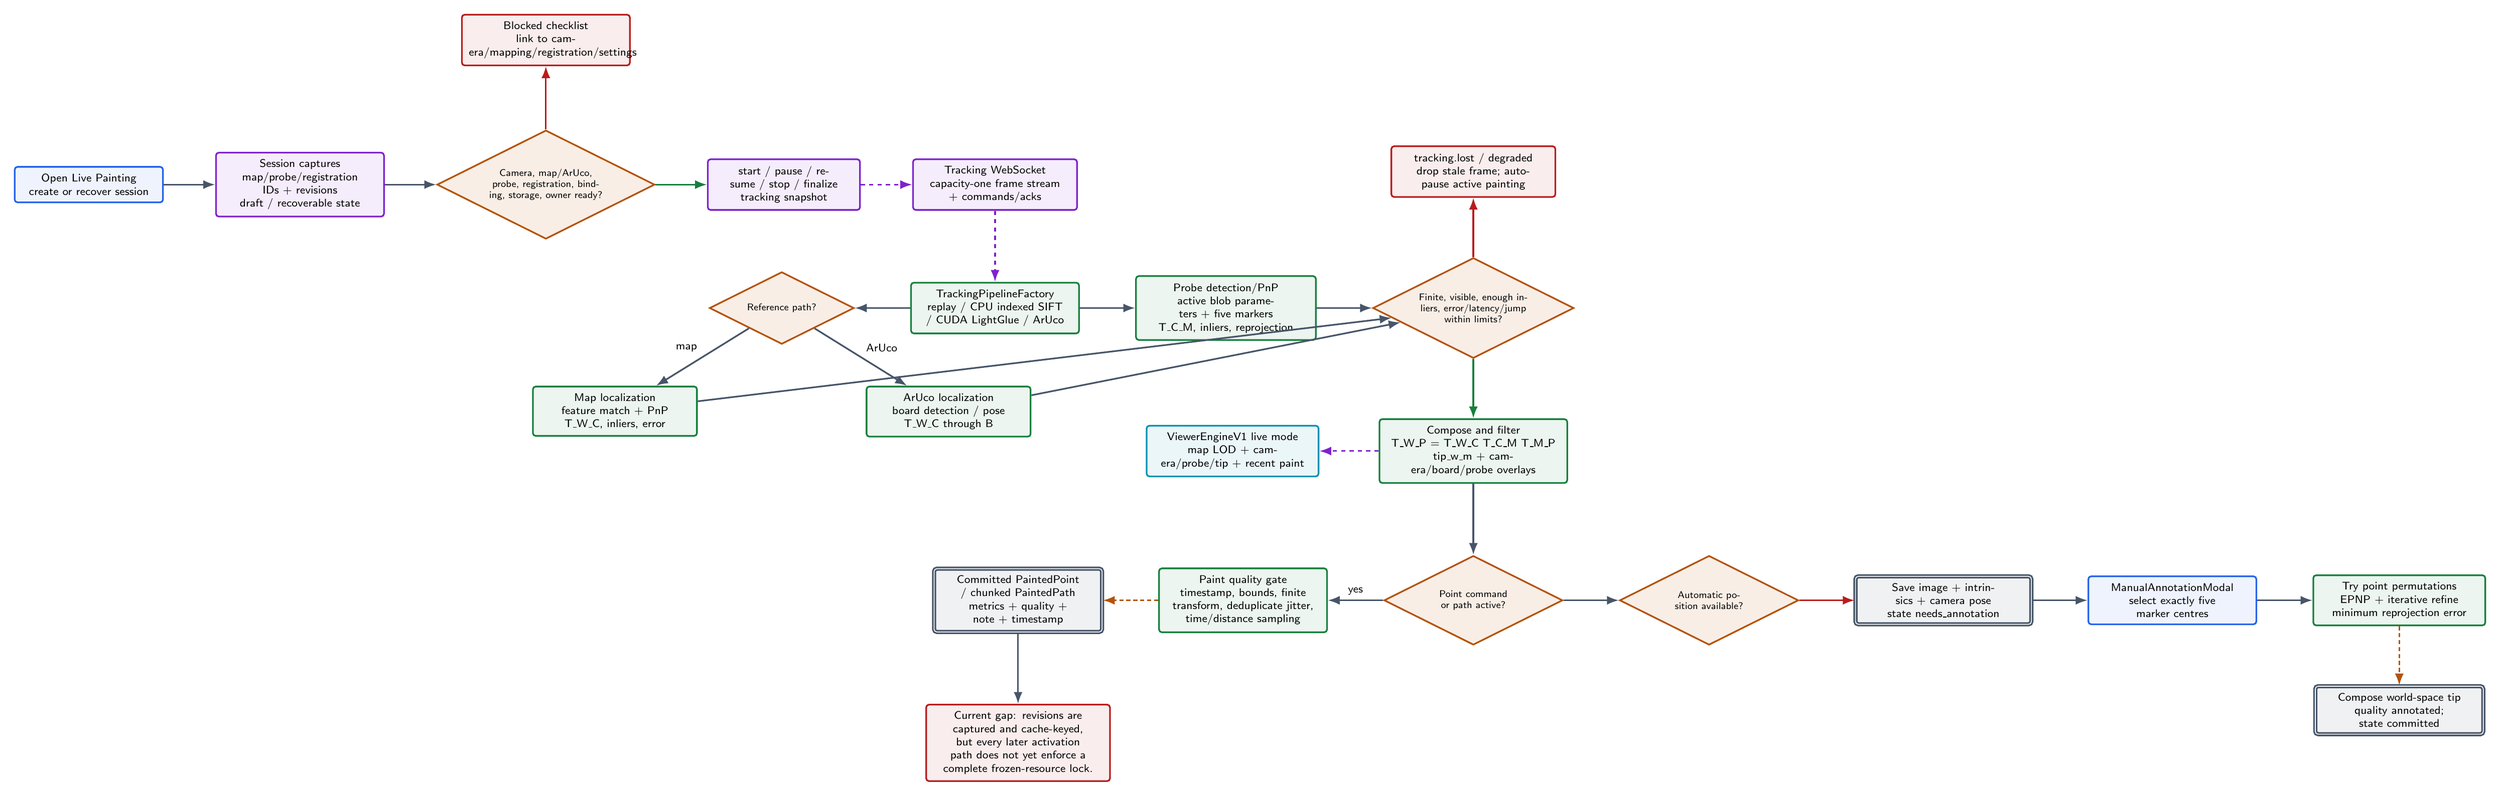
\begin{tikzpicture}[node distance=9mm and 12mm]
\node[user,text width=34mm] (live) {Open Live Painting\\create or recover session};
\node[api,text width=39mm,right=13mm of live] (session) {Session captures map/probe/registration IDs + revisions\\draft / recoverable state};
\node[decision,text width=35mm,right=13mm of session] (preflight) {Camera, map/ArUco, probe, registration, binding, storage, owner ready?};
\node[warning,text width=39mm,above=16mm of preflight] (blocked) {Blocked checklist\\link to camera/mapping/registration/settings};
\node[api,text width=35mm,right=13mm of preflight] (start) {start / pause / resume / stop / finalize\\tracking snapshot};
\node[api,text width=38mm,right=13mm of start] (ws) {Tracking WebSocket\\capacity-one frame stream + commands/acks};

\node[service,text width=39mm,below=18mm of ws] (factory) {TrackingPipelineFactory\\replay / CPU indexed SIFT / CUDA LightGlue / ArUco};
\node[decision,text width=28mm,left=14mm of factory] (refmode) {Reference path?};
\node[service,text width=38mm,below left=15mm and 12mm of refmode] (maploc) {Map localization\\feature match + PnP\\T\_W\_C, inliers, error};
\node[service,text width=38mm,below right=15mm and 12mm of refmode] (boardloc) {ArUco localization\\board detection / pose\\T\_W\_C through B};
\node[service,text width=42mm,right=14mm of factory] (probepnp) {Probe detection/PnP\\active blob parameters + five markers\\T\_C\_M, inliers, reprojection};
\node[decision,text width=32mm,right=14mm of probepnp] (quality) {Finite, visible, enough inliers, error/latency/jump within limits?};
\node[warning,text width=38mm,above=15mm of quality] (lost) {tracking.lost / degraded\\drop stale frame; auto-pause active painting};
\node[service,text width=44mm,below=15mm of quality] (compose) {Compose and filter\\T\_W\_P = T\_W\_C T\_C\_M T\_M\_P\\tip\_w\_m + camera/board/probe overlays};

\node[page,text width=40mm,left=15mm of compose] (viewer) {ViewerEngineV1 live mode\\map LOD + camera/probe/tip + recent paint};
\node[decision,text width=31mm,below=18mm of compose] (paintmode) {Point command or path active?};
\node[service,text width=39mm,left=14mm of paintmode] (gate) {Paint quality gate\\timestamp, bounds, finite transform, deduplicate jitter, time/distance sampling};
\node[data,text width=39mm,left=14mm of gate] (record) {Committed PaintedPoint / chunked PaintedPath\\metrics + quality + note + timestamp};
\node[decision,text width=32mm,right=14mm of paintmode] (tracked) {Automatic position available?};
\node[data,text width=41mm,right=14mm of tracked] (image) {Save image + intrinsics + camera pose\\state needs\_annotation};
\node[user,text width=39mm,right=14mm of image] (manual) {ManualAnnotationModal\\select exactly five marker centres};
\node[service,text width=40mm,right=14mm of manual] (manualpnp) {Try point permutations\\EPNP + iterative refine\\minimum reprojection error};
\node[data,text width=39mm,below=15mm of manualpnp] (resolved) {Compose world-space tip\\quality annotated; state committed};

\node[warning,text width=43mm,below=18mm of record] (frozengap) {Current gap: revisions are captured and cache-keyed, but every later activation path does not yet enforce a complete frozen-resource lock.};

\draw[flow] (live) -- (session);
\draw[flow] (session) -- (preflight);
\draw[no] (preflight) -- (blocked);
\draw[yes] (preflight) -- (start);
\draw[event] (start) -- (ws);
\draw[event] (ws) -- (factory);
\draw[flow] (factory) -- (refmode);
\draw[flow] (refmode) -- node[above left]{map} (maploc);
\draw[flow] (refmode) -- node[above right]{ArUco} (boardloc);
\draw[flow] (factory) -- (probepnp);
\draw[flow] (maploc) -- (quality);
\draw[flow] (boardloc) -- (quality);
\draw[flow] (probepnp) -- (quality);
\draw[no] (quality) -- (lost);
\draw[yes] (quality) -- (compose);
\draw[event] (compose) -- (viewer);
\draw[flow] (compose) -- (paintmode);
\draw[flow] (paintmode) -- node[above]{yes} (gate);
\draw[artifact] (gate) -- (record);
\draw[flow] (paintmode) -- (tracked);
\draw[no] (tracked) -- (image);
\draw[flow] (image) -- (manual);
\draw[flow] (manual) -- (manualpnp);
\draw[artifact] (manualpnp) -- (resolved);
\draw[flow] (record) -- (frozengap);
\end{tikzpicture}}
\newpage

% -----------------------------------------------------------------------------
\flowtitle{8. Session review, replay, record editing, manual annotation, and exports}{Server records remain authoritative}
\resizebox{\textwidth}{0.82\textheight}{%
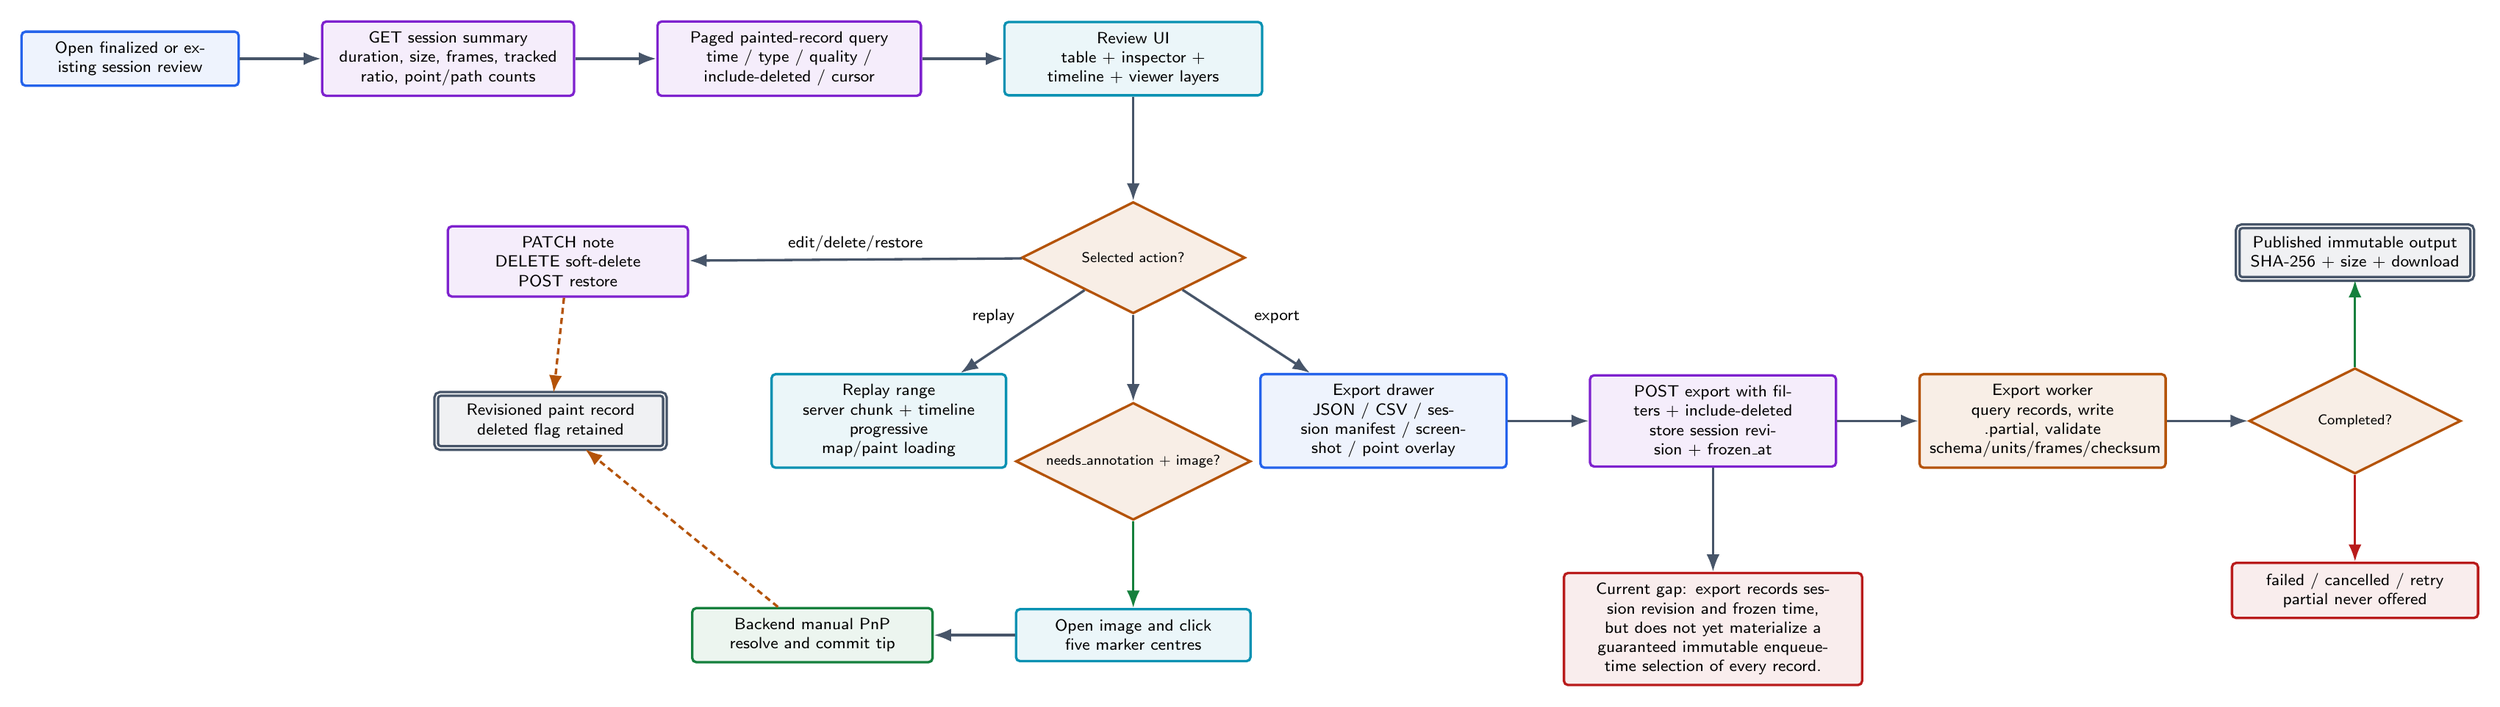
\begin{tikzpicture}[node distance=10mm and 13mm]
\node[user,text width=34mm] (open) {Open finalized or existing session review};
\node[api,text width=40mm,right=14mm of open] (summary) {GET session summary\\duration, size, frames, tracked ratio, point/path counts};
\node[api,text width=42mm,right=14mm of summary] (query) {Paged painted-record query\\time / type / quality / include-deleted / cursor};
\node[page,text width=41mm,right=14mm of query] (review) {Review UI\\table + inspector + timeline + viewer layers};

\node[decision,text width=31mm,below=18mm of review] (action) {Selected action?};
\node[page,text width=37mm,below left=15mm and 12mm of action] (replay) {Replay range\\server chunk + timeline\\progressive map/paint loading};
\node[api,text width=38mm,above left=13mm and 14mm of replay] (edit) {PATCH note\\DELETE soft-delete\\POST restore};
\node[data,text width=36mm,left=18mm of replay] (record) {Revisioned paint record\\deleted flag retained};

\node[decision,text width=32mm,below=15mm of action] (needs) {needs\_annotation + image?};
\node[page,text width=37mm,below=15mm of needs] (annotate) {Open image and click five marker centres};
\node[service,text width=38mm,left=14mm of annotate] (pnp) {Backend manual PnP\\resolve and commit tip};

\node[user,text width=39mm,below right=15mm and 12mm of action] (exportui) {Export drawer\\JSON / CSV / session manifest / screenshot / point overlay};
\node[api,text width=39mm,right=14mm of exportui] (exportapi) {POST export with filters + include-deleted\\store session revision + frozen\_at};
\node[worker,text width=39mm,right=14mm of exportapi] (exportworker) {Export worker\\query records, write .partial, validate schema/units/frames/checksum};
\node[decision,text width=28mm,right=14mm of exportworker] (done) {Completed?};
\node[data,text width=37mm,above=15mm of done] (download) {Published immutable output\\SHA-256 + size + download};
\node[warning,text width=39mm,below=15mm of done] (retry) {failed / cancelled / retry\\partial never offered};
\node[warning,text width=48mm,below=18mm of exportapi] (snapshotgap) {Current gap: export records session revision and frozen time, but does not yet materialize a guaranteed immutable enqueue-time selection of every record.};

\draw[flow] (open) -- (summary);
\draw[flow] (summary) -- (query);
\draw[flow] (query) -- (review);
\draw[flow] (review) -- (action);
\draw[flow] (action) -- node[above left]{replay} (replay);
\draw[flow] (action) -- node[above]{edit/delete/restore} (edit);
\draw[artifact] (edit) -- (record);
\draw[flow] (action) -- (needs);
\draw[yes] (needs) -- (annotate);
\draw[flow] (annotate) -- (pnp);
\draw[artifact] (pnp) -- (record);
\draw[flow] (action) -- node[above right]{export} (exportui);
\draw[flow] (exportui) -- (exportapi);
\draw[flow] (exportapi) -- (exportworker);
\draw[flow] (exportworker) -- (done);
\draw[yes] (done) -- (download);
\draw[no] (done) -- (retry);
\draw[flow] (exportapi) -- (snapshotgap);
\end{tikzpicture}}
\newpage

% -----------------------------------------------------------------------------
\flowtitle{9. Durable jobs, cancellation, recovery, and atomic publication}{Mapping, export, legacy import, repair, support, and migration share supervision}
\resizebox{\textwidth}{0.82\textheight}{%
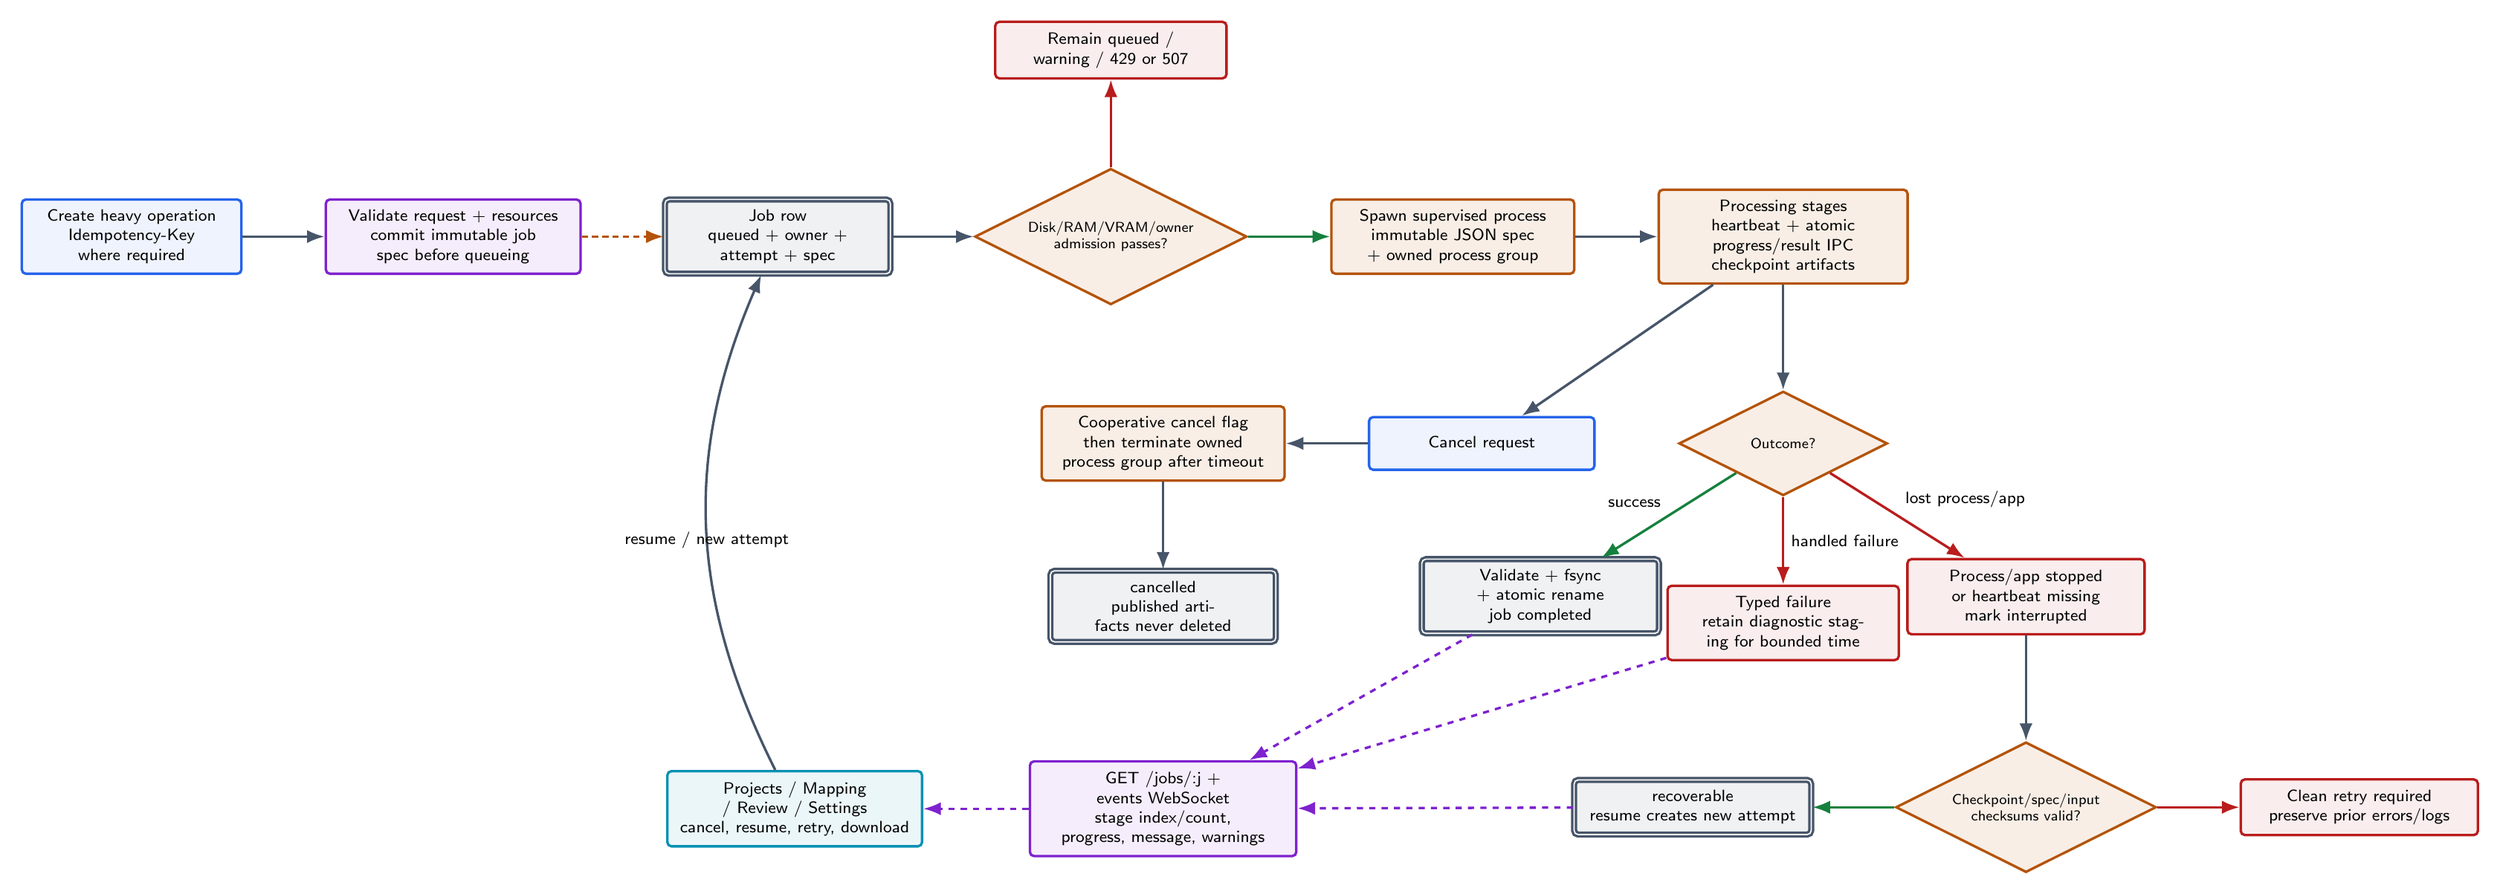
\begin{tikzpicture}[node distance=10mm and 13mm]
\node[user,text width=34mm] (command) {Create heavy operation\\Idempotency-Key where required};
\node[api,text width=40mm,right=14mm of command] (spec) {Validate request + resources\\commit immutable job spec before queueing};
\node[data,text width=35mm,right=14mm of spec] (jobrow) {Job row\\queued + owner + attempt + spec};
\node[decision,text width=32mm,right=14mm of jobrow] (admission) {Disk/RAM/VRAM/owner admission passes?};
\node[warning,text width=36mm,above=15mm of admission] (wait) {Remain queued / warning / 429 or 507};
\node[worker,text width=38mm,right=14mm of admission] (spawn) {Spawn supervised process\\immutable JSON spec + owned process group};
\node[worker,text width=39mm,right=14mm of spawn] (work) {Processing stages\\heartbeat + atomic progress/result IPC\\checkpoint artifacts};

\node[decision,text width=28mm,below=18mm of work] (outcome) {Outcome?};
\node[data,text width=37mm,below left=15mm and 12mm of outcome] (complete) {Validate + fsync + atomic rename\\job completed};
\node[warning,text width=36mm,below=15mm of outcome] (failed) {Typed failure\\retain diagnostic staging for bounded time};
\node[warning,text width=37mm,below right=15mm and 12mm of outcome] (interrupted) {Process/app stopped or heartbeat missing\\mark interrupted};

\node[user,text width=35mm,left=14mm of outcome] (cancel) {Cancel request};
\node[worker,text width=38mm,left=14mm of cancel] (coop) {Cooperative cancel flag\\then terminate owned process group after timeout};
\node[data,text width=35mm,below=15mm of coop] (cancelled) {cancelled\\published artifacts never deleted};

\node[decision,text width=31mm,below=18mm of interrupted] (checkpoint) {Checkpoint/spec/input checksums valid?};
\node[data,text width=37mm,left=14mm of checkpoint] (recoverable) {recoverable\\resume creates new attempt};
\node[warning,text width=37mm,right=14mm of checkpoint] (cleanretry) {Clean retry required\\preserve prior errors/logs};

\node[api,text width=42mm,below=20mm of cancelled] (events) {GET /jobs/:j + events WebSocket\\stage index/count, progress, message, warnings};
\node[page,text width=40mm,left=18mm of events] (ui) {Projects / Mapping / Review / Settings\\cancel, resume, retry, download};

\draw[flow] (command) -- (spec);
\draw[artifact] (spec) -- (jobrow);
\draw[flow] (jobrow) -- (admission);
\draw[no] (admission) -- (wait);
\draw[yes] (admission) -- (spawn);
\draw[flow] (spawn) -- (work);
\draw[flow] (work) -- (outcome);
\draw[yes] (outcome) -- node[above left]{success} (complete);
\draw[no] (outcome) -- node[right]{handled failure} (failed);
\draw[no] (outcome) -- node[above right]{lost process/app} (interrupted);
\draw[flow] (work) -- (cancel);
\draw[flow] (cancel) -- (coop);
\draw[flow] (coop) -- (cancelled);
\draw[flow] (interrupted) -- (checkpoint);
\draw[yes] (checkpoint) -- (recoverable);
\draw[no] (checkpoint) -- (cleanretry);
\draw[event] (complete) -- (events);
\draw[event] (failed) -- (events);
\draw[event] (recoverable) -- (events);
\draw[event] (events) -- (ui);
\draw[flow] (ui) to[bend left=25] node[below]{resume / new attempt} (jobrow);
\end{tikzpicture}}
\newpage

% -----------------------------------------------------------------------------
\flowtitle{10. Settings, diagnostics, support, repair, migration, startup, and security}{Operational logic and local-first boundaries}
\resizebox{\textwidth}{0.82\textheight}{%
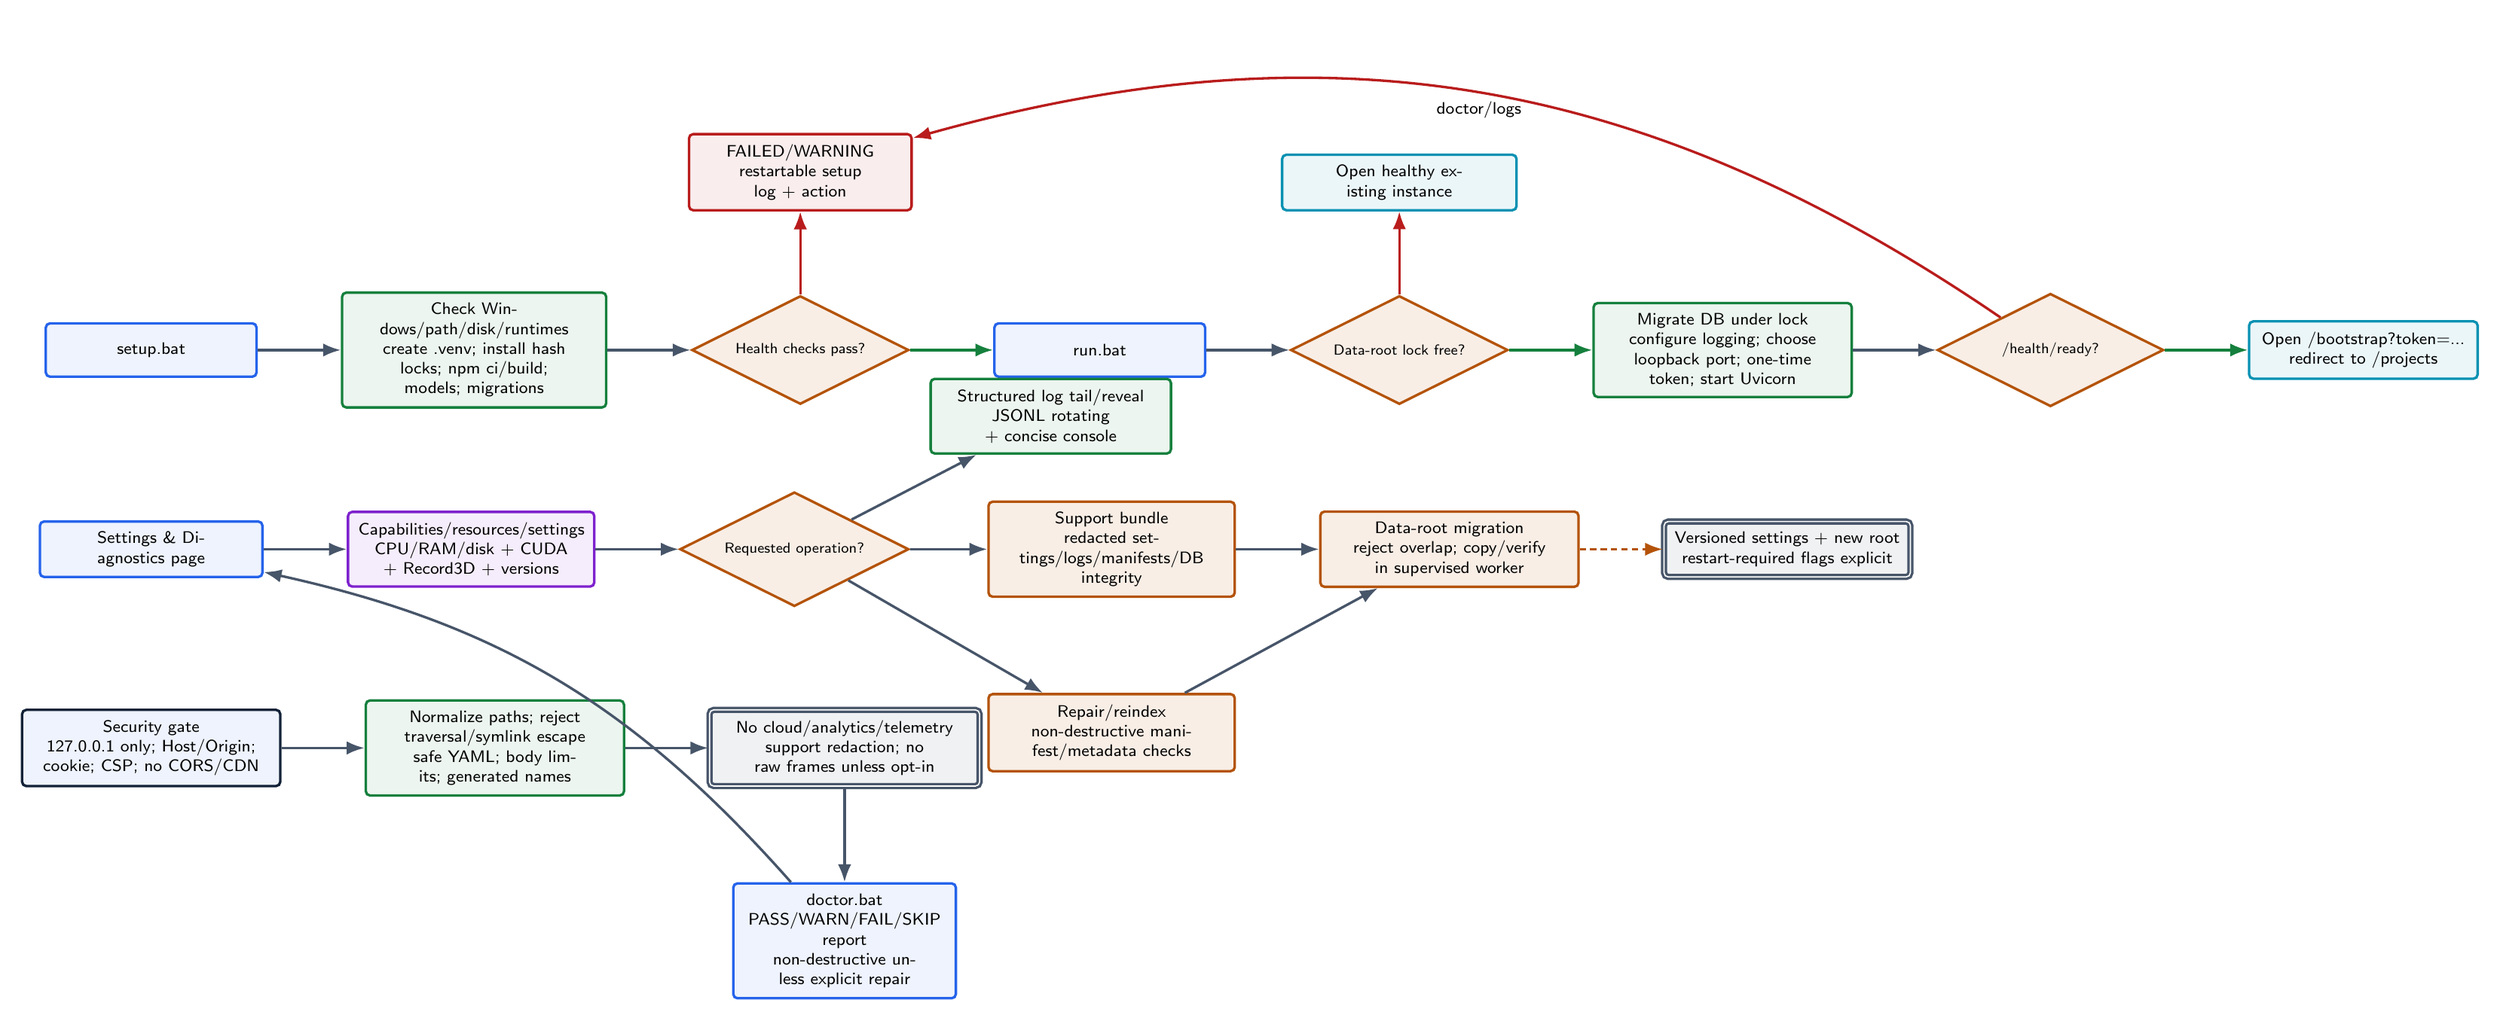
\begin{tikzpicture}[node distance=9mm and 13mm]
\node[user,text width=32mm] (setup) {setup.bat};
\node[service,text width=41mm,right=14mm of setup] (bootstrap) {Check Windows/path/disk/runtimes\\create .venv; install hash locks; npm ci/build; models; migrations};
\node[decision,text width=28mm,right=14mm of bootstrap] (setupok) {Health checks pass?};
\node[warning,text width=34mm,above=14mm of setupok] (setuplog) {FAILED/WARNING\\restartable setup log + action};
\node[user,text width=32mm,right=14mm of setupok] (run) {run.bat};
\node[decision,text width=29mm,right=14mm of run] (lock) {Data-root lock free?};
\node[page,text width=36mm,above=14mm of lock] (existing) {Open healthy existing instance};
\node[service,text width=40mm,right=14mm of lock] (startup) {Migrate DB under lock\\configure logging; choose loopback port; one-time token; start Uvicorn};
\node[decision,text width=29mm,right=14mm of startup] (ready) {/health/ready?};
\node[page,text width=35mm,right=14mm of ready] (browser) {Open /bootstrap?token=...\\redirect to /projects};

\node[user,text width=34mm,below=24mm of setup] (settings) {Settings \& Diagnostics page};
\node[api,text width=38mm,right=14mm of settings] (caps) {Capabilities/resources/settings\\CPU/RAM/disk + CUDA + Record3D + versions};
\node[decision,text width=30mm,right=14mm of caps] (operation) {Requested operation?};
\node[service,text width=37mm,above right=11mm and 13mm of operation] (logs) {Structured log tail/reveal\\JSONL rotating + concise console};
\node[worker,text width=38mm,right=13mm of operation] (support) {Support bundle\\redacted settings/logs/manifests/DB integrity};
\node[worker,text width=38mm,below=16mm of support] (repair) {Repair/reindex\\non-destructive manifest/metadata checks};
\node[worker,text width=40mm,right=14mm of support] (migration) {Data-root migration\\reject overlap; copy/verify in supervised worker};
\node[data,text width=38mm,right=14mm of migration] (settingsdata) {Versioned settings + new root\\restart-required flags explicit};

\node[hardware,text width=40mm,below=22mm of settings] (security) {Security gate\\127.0.0.1 only; Host/Origin; cookie; CSP; no CORS/CDN};
\node[service,text width=40mm,right=14mm of security] (paths) {Normalize paths; reject traversal/symlink escape\\safe YAML; body limits; generated names};
\node[data,text width=42mm,right=14mm of paths] (privacy) {No cloud/analytics/telemetry\\support redaction; no raw frames unless opt-in};
\node[user,text width=34mm,below=16mm of privacy] (doctor) {doctor.bat\\PASS/WARN/FAIL/SKIP report\\non-destructive unless explicit repair};

\draw[flow] (setup) -- (bootstrap);
\draw[flow] (bootstrap) -- (setupok);
\draw[no] (setupok) -- (setuplog);
\draw[yes] (setupok) -- (run);
\draw[flow] (run) -- (lock);
\draw[no] (lock) -- (existing);
\draw[yes] (lock) -- (startup);
\draw[flow] (startup) -- (ready);
\draw[yes] (ready) -- (browser);
\draw[no] (ready) to[bend right=25] node[below]{doctor/logs} (setuplog);
\draw[flow] (settings) -- (caps);
\draw[flow] (caps) -- (operation);
\draw[flow] (operation) -- (logs);
\draw[flow] (operation) -- (support);
\draw[flow] (operation) -- (repair);
\draw[flow] (support) -- (migration);
\draw[flow] (repair) -- (migration);
\draw[artifact] (migration) -- (settingsdata);
\draw[flow] (security) -- (paths);
\draw[flow] (paths) -- (privacy);
\draw[flow] (privacy) -- (doctor);
\draw[flow] (doctor) to[bend right=18] (settings);
\end{tikzpicture}}
\newpage

% -----------------------------------------------------------------------------
\flowtitle{11. Persistence, domain relationships, revisions, and coordinate transforms}{SQLite owns identity/state; files own large immutable artifacts}
\resizebox{\textwidth}{0.82\textheight}{%
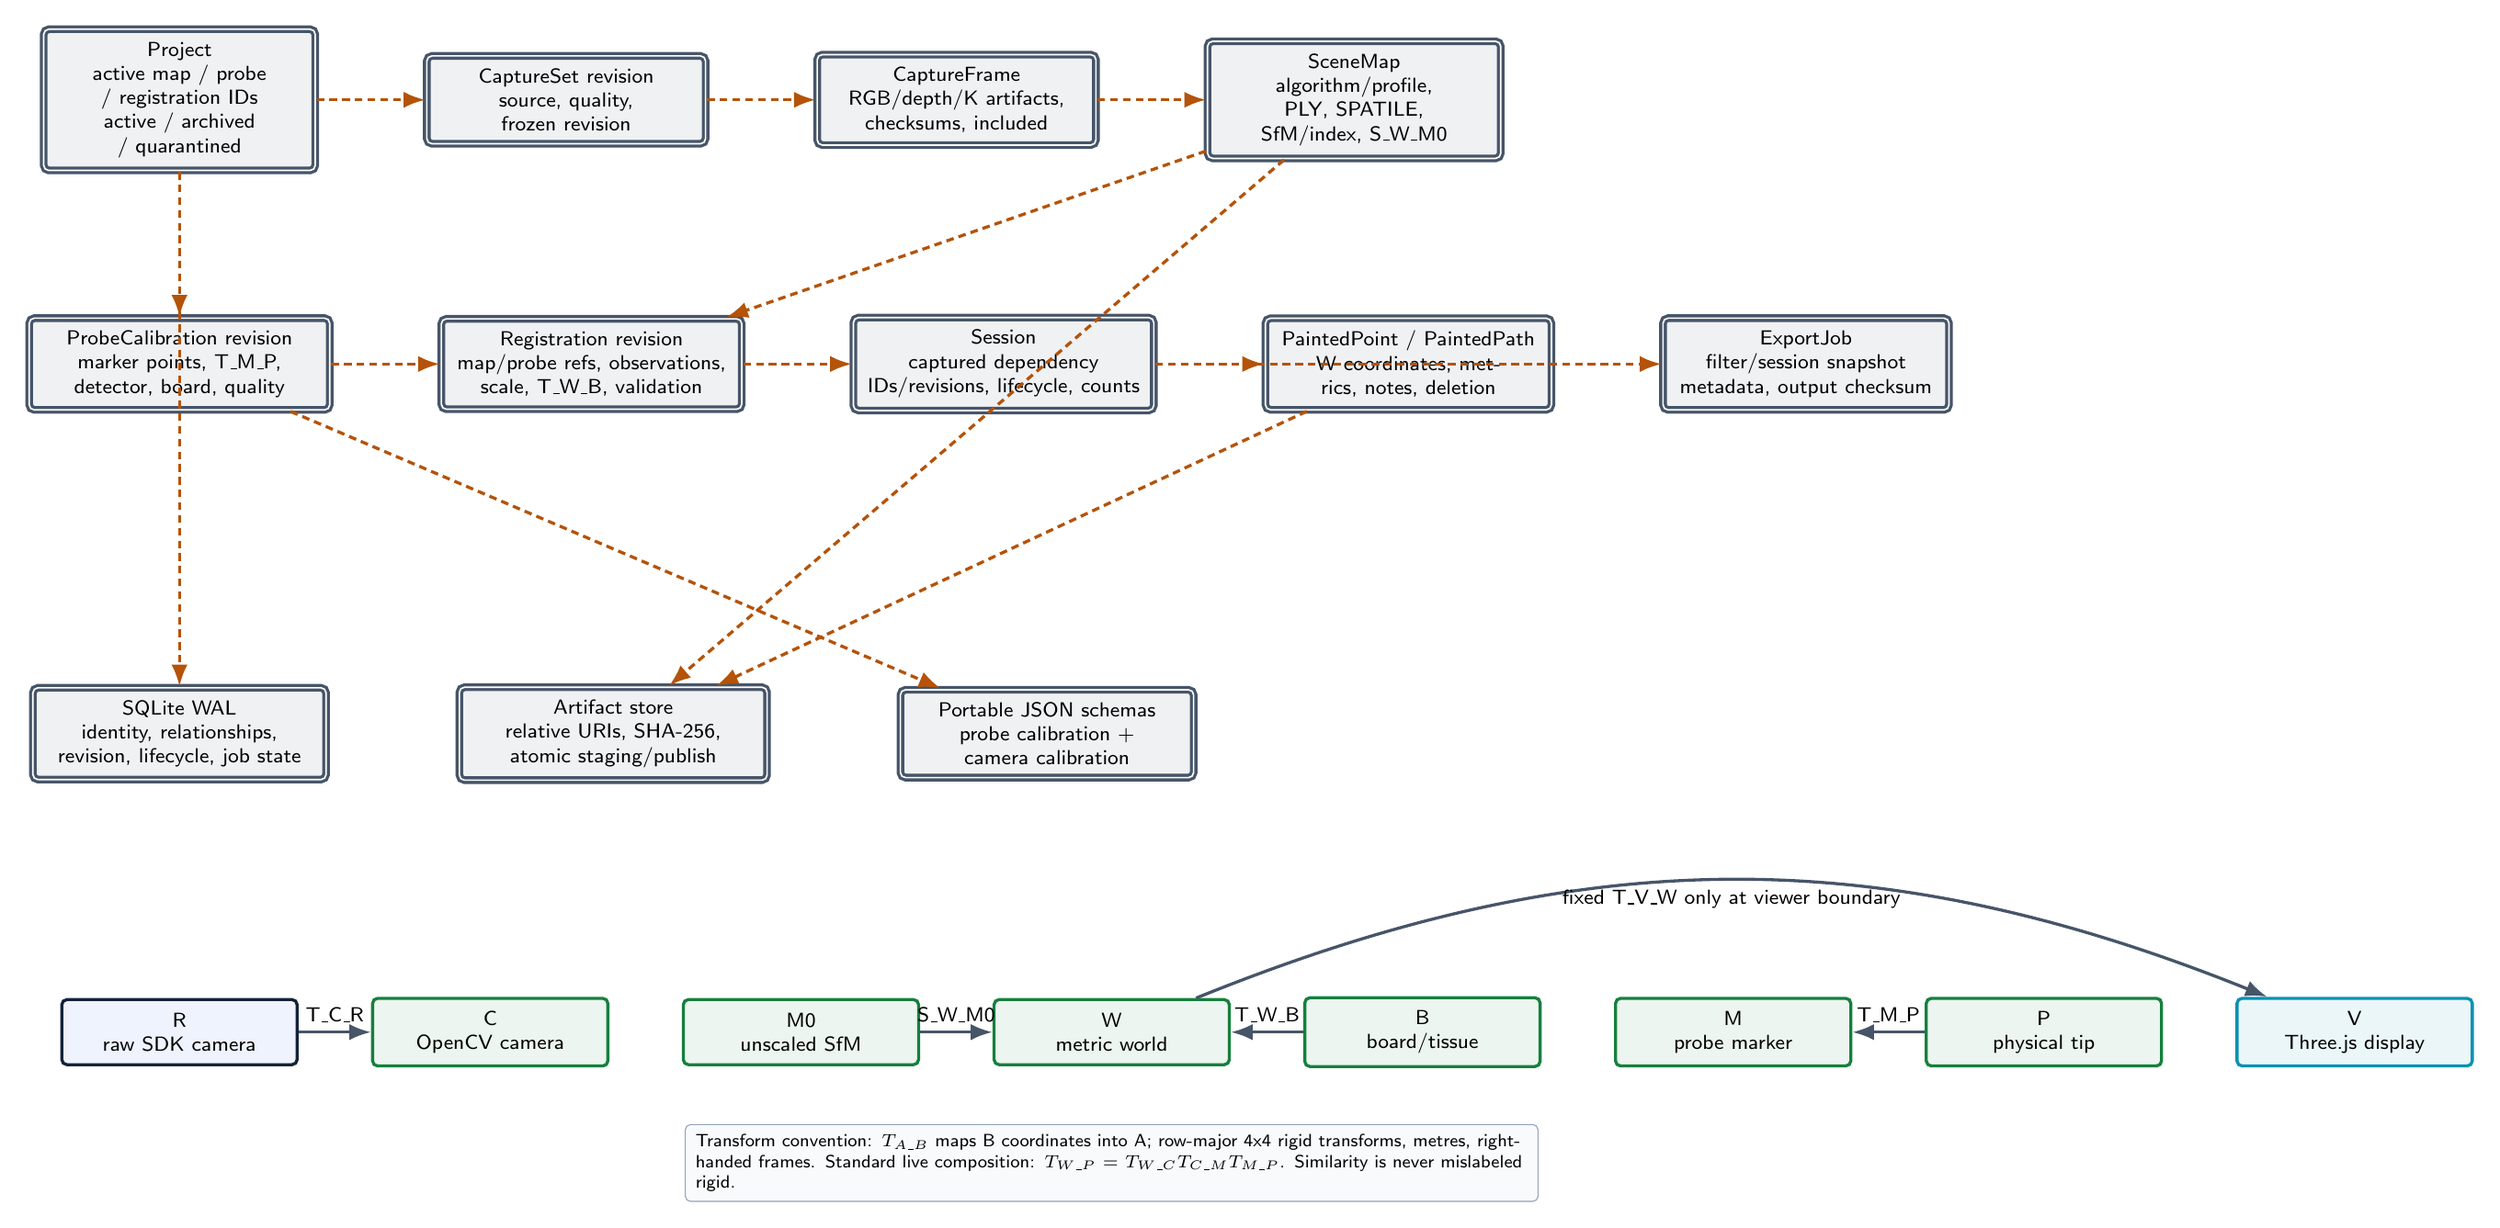
\begin{tikzpicture}[node distance=10mm and 13mm]
\node[data,text width=34mm] (project) {Project\\active map / probe / registration IDs\\active / archived / quarantined};
\node[data,text width=35mm,right=15mm of project] (captureset) {CaptureSet revision\\source, quality, frozen revision};
\node[data,text width=35mm,right=15mm of captureset] (frame) {CaptureFrame\\RGB/depth/K artifacts, checksums, included};
\node[data,text width=37mm,right=15mm of frame] (map) {SceneMap\\algorithm/profile, PLY, SPATILE, SfM/index, S\_W\_M0};

\node[data,text width=38mm,below=20mm of project] (probe) {ProbeCalibration revision\\marker points, T\_M\_P, detector, board, quality};
\node[data,text width=38mm,right=15mm of probe] (registration) {Registration revision\\map/probe refs, observations, scale, T\_W\_B, validation};
\node[data,text width=38mm,right=15mm of registration] (session) {Session\\captured dependency IDs/revisions, lifecycle, counts};
\node[data,text width=36mm,right=15mm of session] (paint) {PaintedPoint / PaintedPath\\W coordinates, metrics, notes, deletion};
\node[data,text width=36mm,right=15mm of paint] (export) {ExportJob\\filter/session snapshot metadata, output checksum};

\node[data,text width=37mm,below=38mm of probe] (sqlite) {SQLite WAL\\identity, relationships, revision, lifecycle, job state};
\node[data,text width=39mm,right=18mm of sqlite] (files) {Artifact store\\relative URIs, SHA-256, atomic staging/publish};
\node[data,text width=37mm,right=18mm of files] (portable) {Portable JSON schemas\\probe calibration + camera calibration};

\node[hardware,text width=29mm,below=30mm of sqlite] (R) {R\\raw SDK camera};
\node[service,text width=29mm,right=10mm of R] (C) {C\\OpenCV camera};
\node[service,text width=29mm,right=10mm of C] (M0) {M0\\unscaled SfM};
\node[service,text width=29mm,right=10mm of M0] (W) {W\\metric world};
\node[service,text width=29mm,right=10mm of W] (B) {B\\board/tissue};
\node[service,text width=29mm,right=10mm of B] (M) {M\\probe marker};
\node[service,text width=29mm,right=10mm of M] (P) {P\\physical tip};
\node[page,text width=29mm,right=10mm of P] (V) {V\\Three.js display};

\draw[artifact] (project) -- (captureset);
\draw[artifact] (captureset) -- (frame);
\draw[artifact] (frame) -- (map);
\draw[artifact] (project) -- (probe);
\draw[artifact] (map) -- (registration);
\draw[artifact] (probe) -- (registration);
\draw[artifact] (registration) -- (session);
\draw[artifact] (session) -- (paint);
\draw[artifact] (session) -- (export);
\draw[artifact] (project) -- (sqlite);
\draw[artifact] (map) -- (files);
\draw[artifact] (paint) -- (files);
\draw[artifact] (probe) -- (portable);
\draw[flow] (R) -- node[above]{T\_C\_R} (C);
\draw[flow] (M0) -- node[above]{S\_W\_M0} (W);
\draw[flow] (B) -- node[above]{T\_W\_B} (W);
\draw[flow] (P) -- node[above]{T\_M\_P} (M);
\draw[flow] (W) to[bend left=22] node[below]{fixed T\_V\_W only at viewer boundary} (V);
\node[note,text width=115mm,below=8mm of W] {Transform convention: $T_{A\_B}$ maps B coordinates into A; row-major 4x4 rigid transforms, metres, right-handed frames. Standard live composition: $T_{W\_P}=T_{W\_C}T_{C\_M}T_{M\_P}$. Similarity is never mislabeled rigid.};
\end{tikzpicture}}
\newpage

% -----------------------------------------------------------------------------
\flowtitle{12. API, WebSocket, and function coverage index}{Every current user-visible domain is represented in pages 1--11}
\small
\begin{tabularx}{\textwidth}{>{\bfseries}p{30mm} X X p{34mm}}
\toprule
Domain & REST functions & Stream / internal logic & Flow pages \\
\midrule
System & live/ready health; capabilities; resources; diagnostics; settings get/patch & startup lock, CUDA probe, logging, resource admission & 1, 9, 10 \\
Projects & list/create/get/rename; summary; clone; archive/restore; reveal; jobs & project selection, readiness, warnings, legacy import & 2, 9, 11 \\
Camera & devices/status; connect/disconnect & preview WS; exclusive owner; normalized capacity-one frames & 3 \\
External calibration & validate/import/get/activate & schema/model/resolution compatibility; preserve original & 3 \\
Capture & sets list/create/get; capture/import; include patch; delete; thumbnail/image & quality, checksums, revision freeze & 3, 4 \\
Maps & list/create/get; transform; align-aruco; activate; manifest/tiles & replay/CPU/CUDA mapping; SPATILE LOD; localization artifacts & 4, 6, 11 \\
Probe calibration & capture/create; validate/import/get/download/activate/revise & probe-test and probe-tuning WS; blob detection; PnP; complete JSON & 5 \\
ArUco calibration & capture/solve; map align & joint board/probe observations; layout and scale optimization & 6 \\
Registration & list/create/get; add/delete/clear observations; solve/validate/activate & registration tracking WS; map/kinematic/ArUco transforms & 6 \\
Sessions & list/create/get; start/pause/resume/stop/finalize; snapshot & tracking WS; frozen refs; lifecycle/reconnect/recovery & 7, 11 \\
Painting & point/path create; recent tracking; undo & quality gate; time/distance sampling; chunks; image fallback & 7 \\
Review & paged records/points/paths; replay; note; delete/restore; image; annotate & viewer filters/timeline; five-point manual PnP & 8 \\
Exports & list/create/download & JSON, CSV, session manifest, screenshot, point overlay; checksum publication & 8, 9 \\
Jobs & get/cancel/resume & events WS; spawn, heartbeat, progress, checkpoint, retry/recovery & 9 \\
Operations & support bundle; repair/reindex; data-root migration; log tail/reveal & supervised operations worker; redaction; overlap checks & 9, 10 \\
Legacy migration & create/status/report & staged import, normalization, validation, untouched source & 1, 9 \\
Viewer & map manifest/tiles and frame images & mapping, registration, live, review modes; LOD; transforms; overlays; disposal & 1, 2, 4, 6--8 \\
\bottomrule
\end{tabularx}

\vspace{5mm}
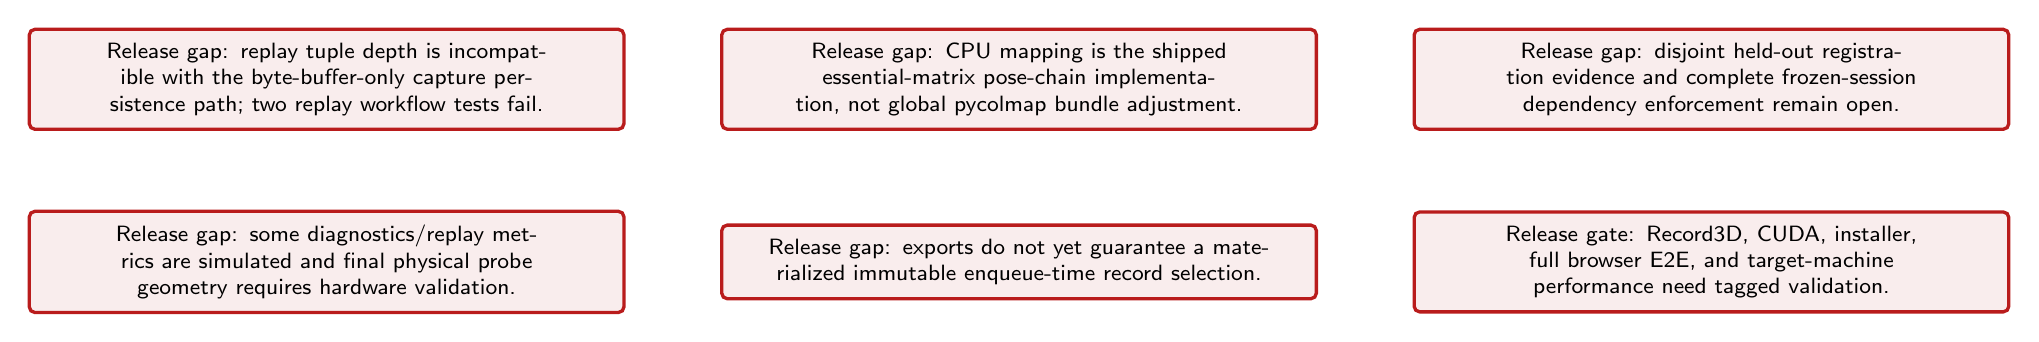
\begin{tikzpicture}[node distance=8mm and 12mm]
\node[warning,text width=72mm] (r1) {Release gap: replay tuple depth is incompatible with the byte-buffer-only capture persistence path; two replay workflow tests fail.};
\node[warning,text width=72mm,right=12mm of r1] (r2) {Release gap: CPU mapping is the shipped essential-matrix pose-chain implementation, not global pycolmap bundle adjustment.};
\node[warning,text width=72mm,right=12mm of r2] (r3) {Release gap: disjoint held-out registration evidence and complete frozen-session dependency enforcement remain open.};
\node[warning,text width=72mm,below=10mm of r1] (r4) {Release gap: some diagnostics/replay metrics are simulated and final physical probe geometry requires hardware validation.};
\node[warning,text width=72mm,right=12mm of r4] (r5) {Release gap: exports do not yet guarantee a materialized immutable enqueue-time record selection.};
\node[warning,text width=72mm,right=12mm of r5] (r6) {Release gate: Record3D, CUDA, installer, full browser E2E, and target-machine performance need tagged validation.};
\end{tikzpicture}

\vfill
\textbf{Source of truth:} \texttt{ARCHITECTURE.md} version 1.1 and the as-built repository at commit \texttt{446831b}. This atlas intentionally includes current limitations rather than presenting unimplemented target behavior as complete.

\end{document}
